\documentclass{article}

\input{Packages}
\usepackage[backend=bibtex, sorting=none]{biblatex}
\addbibresource{bibliography.bib}

\newif\ifpartB
\partBtrue % Uncomment this line for Part B (Full File)
% \partBfalse  % Uncomment this line for Part A (Truncated)


\title{Operation Midnight Hammer: an STK Model}
\author{Claudio Vestini}


\begin{document}

\maketitle

\section{Introduction} \label{sec:intro}

This document reports the modelling of the United States Department of War mission codenamed \emph{Operation Midnight Hammer}, which involved aerial strikes on several Iranian nuclear facilities. The operation was modelled using the Ansys software package Systems Tool Kit (STK)~\cite{STK:2025}. The work was carried out using \texttt{STK 12.10} locally on a Razer Blade 14 (Windows 11) machine. The plots were generated using the \texttt{Report \& Graph Manager} toolbox included in the STK package.

\section{Mission goals \& objectives} \label{sec:mission_goals}

Operation Midnight Hammer (OMH) was a United States-led military strike on Iranian nuclear facilities, executed by the United States Air Force and Navy under the command of United States Central Command. The overall objective of OMH was to ``severely degrade Iran's nuclear weapon infrastructure", according to General John Daniel Caine, chairman of the Joint Chiefs of Staff. The operation was carried out on the 21st and 22nd June 2025 over 37 hours, with most strikes occurring between 02:10 and 02:30 Iran Standard Time on June 22nd (18:40-19:00 EDT on June 21st), as part of the broader Iran-Israel war that began with Israeli strikes on 13 June 2025. The strikes were authorised by President Donald Trump following failed diplomatic efforts, including a proposed 60-day negotiation period announced in February 2025, and amid International Atomic Energy Agency concerns over Iran's uranium enrichment to 60 per cent purity (not far from weapons grade). This marked the first United States offensive action in this conflict and the first attack on Iranian territory since 1988.

\section{Mission concept overview}
\label{sec:mission_overview}

The mission involved 13 B-2 Spirit stealth bombers supported by 112 US aircraft, one US nuclear submarine, and a total of 75 surface-to-surface Tomahawk missiles, 14 GBU-57A/B Massive Ordnance Penetrator (MOP) bombs, and several air-to-surface weapons~\cite{lemay2025midnight}. A central component contributing to the success of the mission was space intelligence, which involved the use of the SBRIS constellation for real-time missile launch detection and cueing, the GPS constellation for navigation and tracking of aircraft and weapons, and several electro-optical LEO satellites for post-strike battle damage assessment (BDA). 

The mission unfolded as follows: at 04:00:00 UTC (00:00 EDT) of January 21st 2025, two packages of B-2 bombers took off from the 509th Bomb Wing at Whiteman Air Force Base, MO. The first package, acting as a decoy, comprised 6 aircraft and headed west to Oklahoma, California, Hawaii, and finally Guam. Its sole objective was to deceive enemy intelligence. The real operational package, comprising 7 B-2 units (each manned by two pilots), headed east on an 18-hour trajectory towards Iran. It traversed the Atlantic Ocean and the Mediterranean Sea, performing a total of 3 mid-air refuellings over international waters enabled by 12 KC-135 Stratotankers. Upon entering Israeli airspace, the seven B-2 aircraft were joined by a support package comprising F-35s, F-22s, and other aircraft to aid the strike operations by neutralising potential Iranian countermeasures (no firings were reported). At roughly 21:00:00 UTC (17:00 EDT), a US submarine supported by Israeli warships stationed in the Persian Gulf fired a total of 75 sub-orbital Tomahawk missiles directed at the Isfahan Nuclear Technology Centre, coordinating the strike with the bombers and attack package. With the Tomahawks still soaring through the sky, at roughly 22:00:00 UTC, the joint flight formation entered Iranian airspace through the Iraqi border. At 22:40:00 UTC (18:40 EDT) on June 21st 2025, the lead B-2 bomber, codenamed Mytee-11, released the first two GBU-57s on the Fordow facility, closely followed by another 10 MOPs plus an additional 2 released on Natanz (2 per aircraft). Simultaneously, all GBU-57 warheads and Tomahawk missiles hit their intended targets, in a window of roughly 20 minutes. By 23:30:00 UTC (19::30 EDT), the B-2 bombers had left Iranian airspace, completely undetected. The aircraft returned to Whiteman AFB from their direction of origin, aided by multiple aerial refuellings, arriving at around 18:30:00 UTC (the total flight time was 37 hours). The mission is summarised in Figure~\ref{fig:omh_flyer}.

\begin{figure}[h]
    \centering
    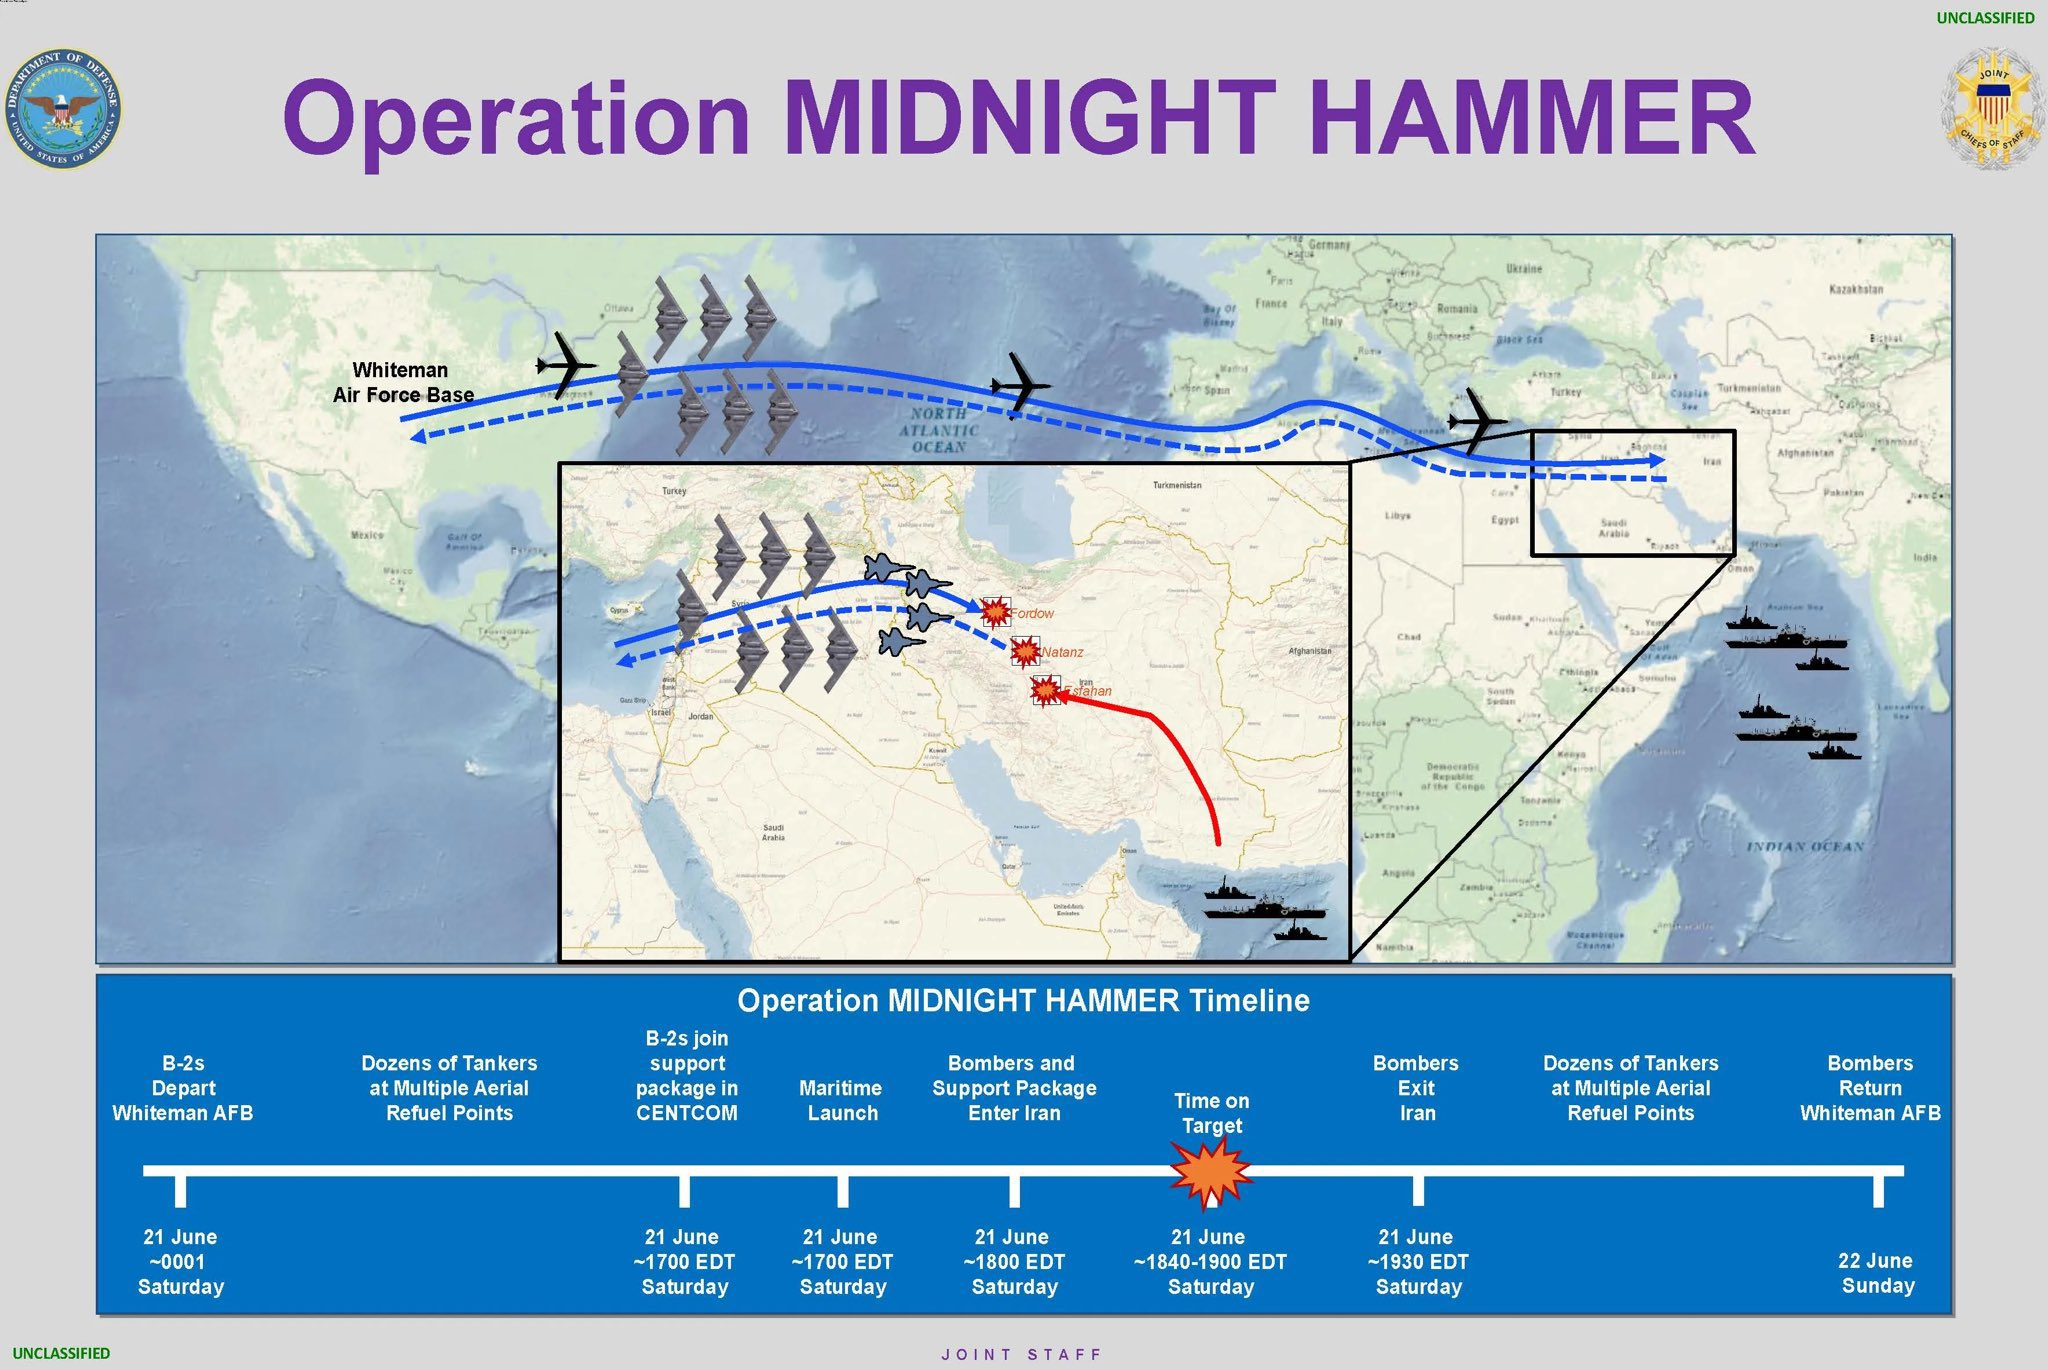
\includegraphics[width=\linewidth]{LaTeX/Figures/Operation_Midnight_Hammer_infographic.jpg}
    \caption{Official Unclassified mission plan for Operation Midnight Hammer (from the DOW).}
    \label{fig:omh_flyer}
\end{figure}

\section{STK model}

The STK model of OMH presented in this report is based on publicly available information, including declassified DOW documents~\cite{lemay2025midnight}, a report by the National Security Space Association (NSSA)~\cite{williams2025midnight}, interviews of army personnel directly and indirectly involved in the operation, and several news outlets reports and reconstructions. Publicly unavailable details were approximated using data from analogous missions, and, throughout the report, we explicitly state when approximations were made. Our model is comprised of a total of 65 individual STK objects, and covers the entire mission timeline through an STK scenario starting on the 21st June 2025 at 04:00:00.000 UTC and ending on the 22nd Jun 2025 at 19:00:00.000 UTC. The model includes the 7 B-2 Spirit live bombers, the 6 decoy B-2 bombers, a total of 6 KC-135 Stratotankers for mid-air refueling, the GBU-57 bombs and Tomahawk missiles, the USS Georgia nuclear submarine and ISN Rahav Israeli ship, several facilities for launch and communications, and a total of 32 satellites and sensors for intelligence and guidance. All figures, source \LaTeX code, source data files and source STK code is made available at the supporting repository:

\begin{center}
    \href{https://github.com/ClouD-161803/MAE341-FinalProject.git}{ClouD-161803/MAE341-FinalProject}.
\end{center}

\subsection{Aircraft and refuelling operations} \label{subsec:aircraft}

A simplified overview of the mission, which hides all components except for the 7 live bombers, all bombs and missiles, the take-off and landing Whiteman Air Force Base in Missouri, the naval infrastructure, and the targets at Fordow, Natanz, and Isfahan, is shown in Figure~\ref{fig:OMH_STK_overview}. This simplified view shows the strike aircraft trajectory (dark blue), which was reconstructed using a total of 534 individual waypoints based on the report at~\cite{lemay2025midnight}. The B-2 Spirit bombers were modelled using STK's built-in \texttt{Aviator} propagator module, which enables the planning of multi-phase aircraft missions involving missile and bomb launches, take-off and landing manoeuvres, and mid-air refuelling operations. The 3D models of the B-2 planes, unavailable natively on STK, were pulled from the FetchCFD website at~\cite{payne_b2spirit_3d} and modified using CAD in Solidworks (using an Oxford University student license) to be made compatible with the STK environment. The 3D model adopted, as well as its appearance in STK, are shown in Figure~\ref{fig:3D_model_B2} and Figure~\ref{fig:B2_model_in_STK}, respectively. The bombers were assumed to cruise at \SI{0.25}{\kilo\metre\per\second} (or 500 knots, which corresponds to Mach 0.85), the B2's optimal operational speed (the speed which minimises fuel usage), at a (reported) altitude of \SI{12}{\kilo\metre}.

\begin{figure}[t]
    \centering
    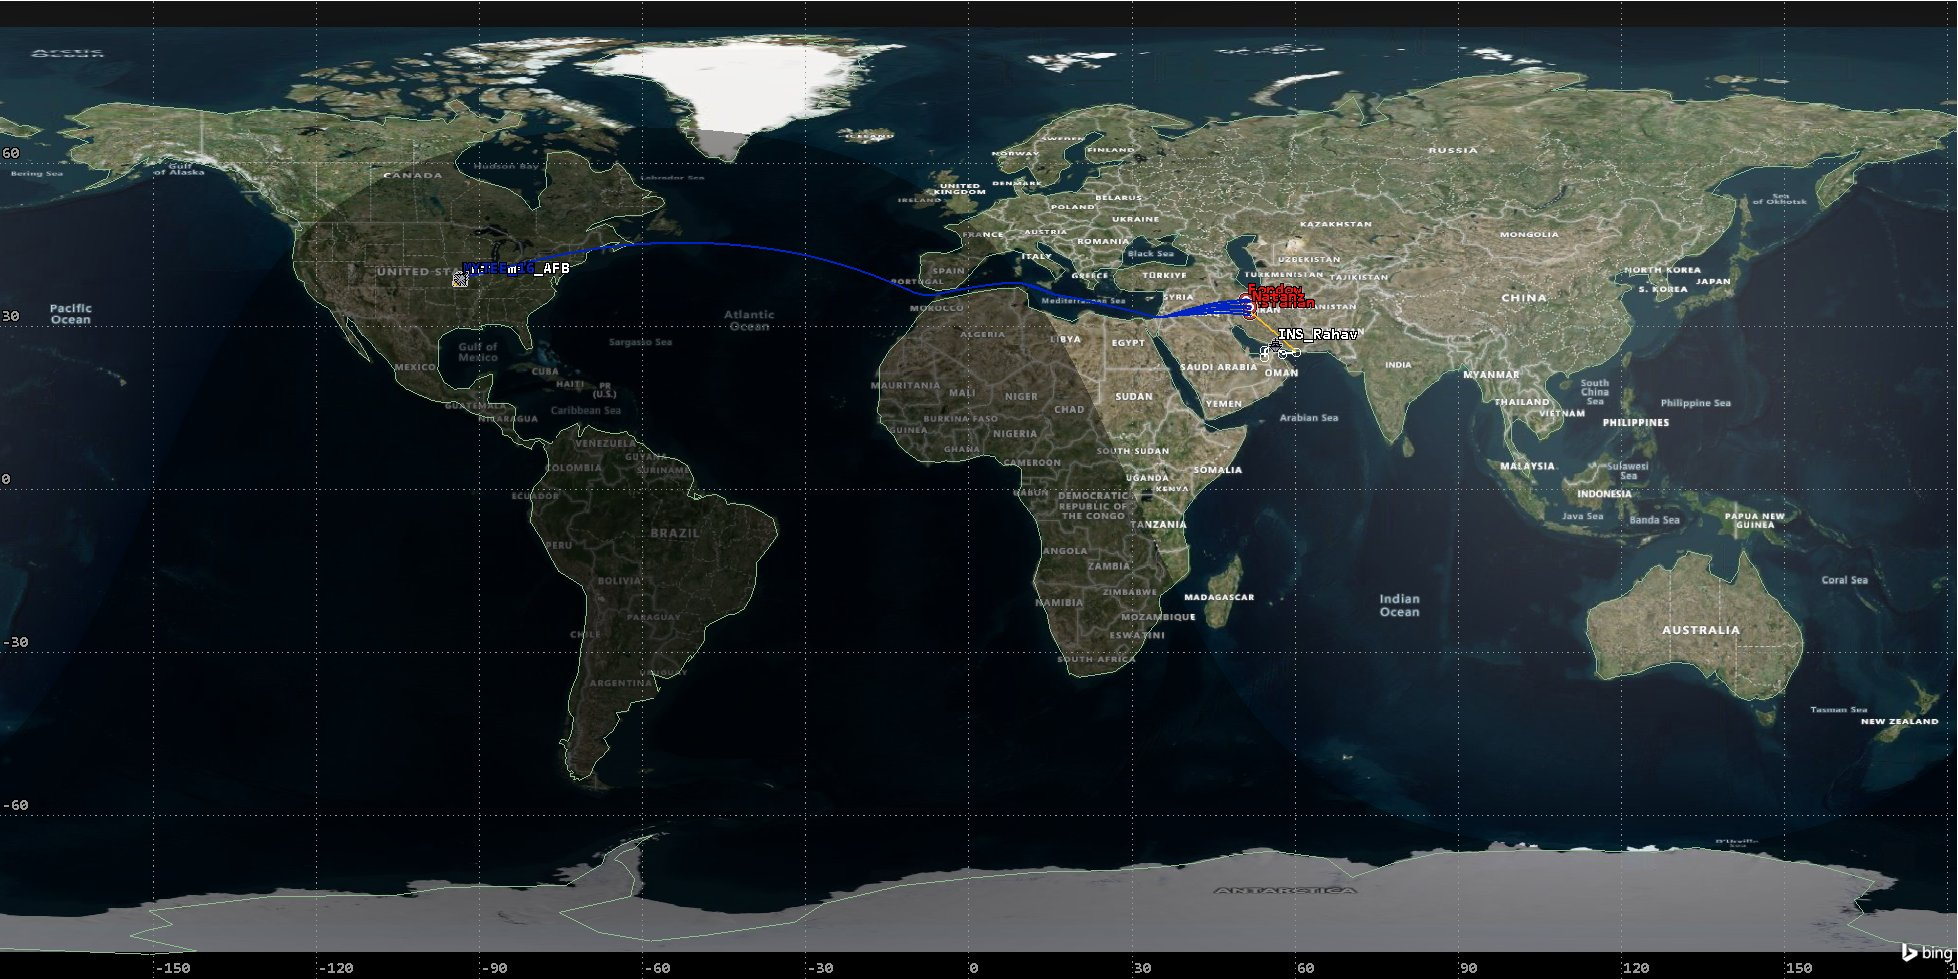
\includegraphics[width=\linewidth]{LaTeX/Figures/Operation_Midnight_Hammer_STK.jpg}
    \caption{Simplified mission overview for Operation Midnight Hammer in STK.v}
    \label{fig:OMH_STK_overview}
\end{figure}

\begin{figure}
    \centering
    \begin{subfigure}[b]{0.68\textwidth}
        \centering
        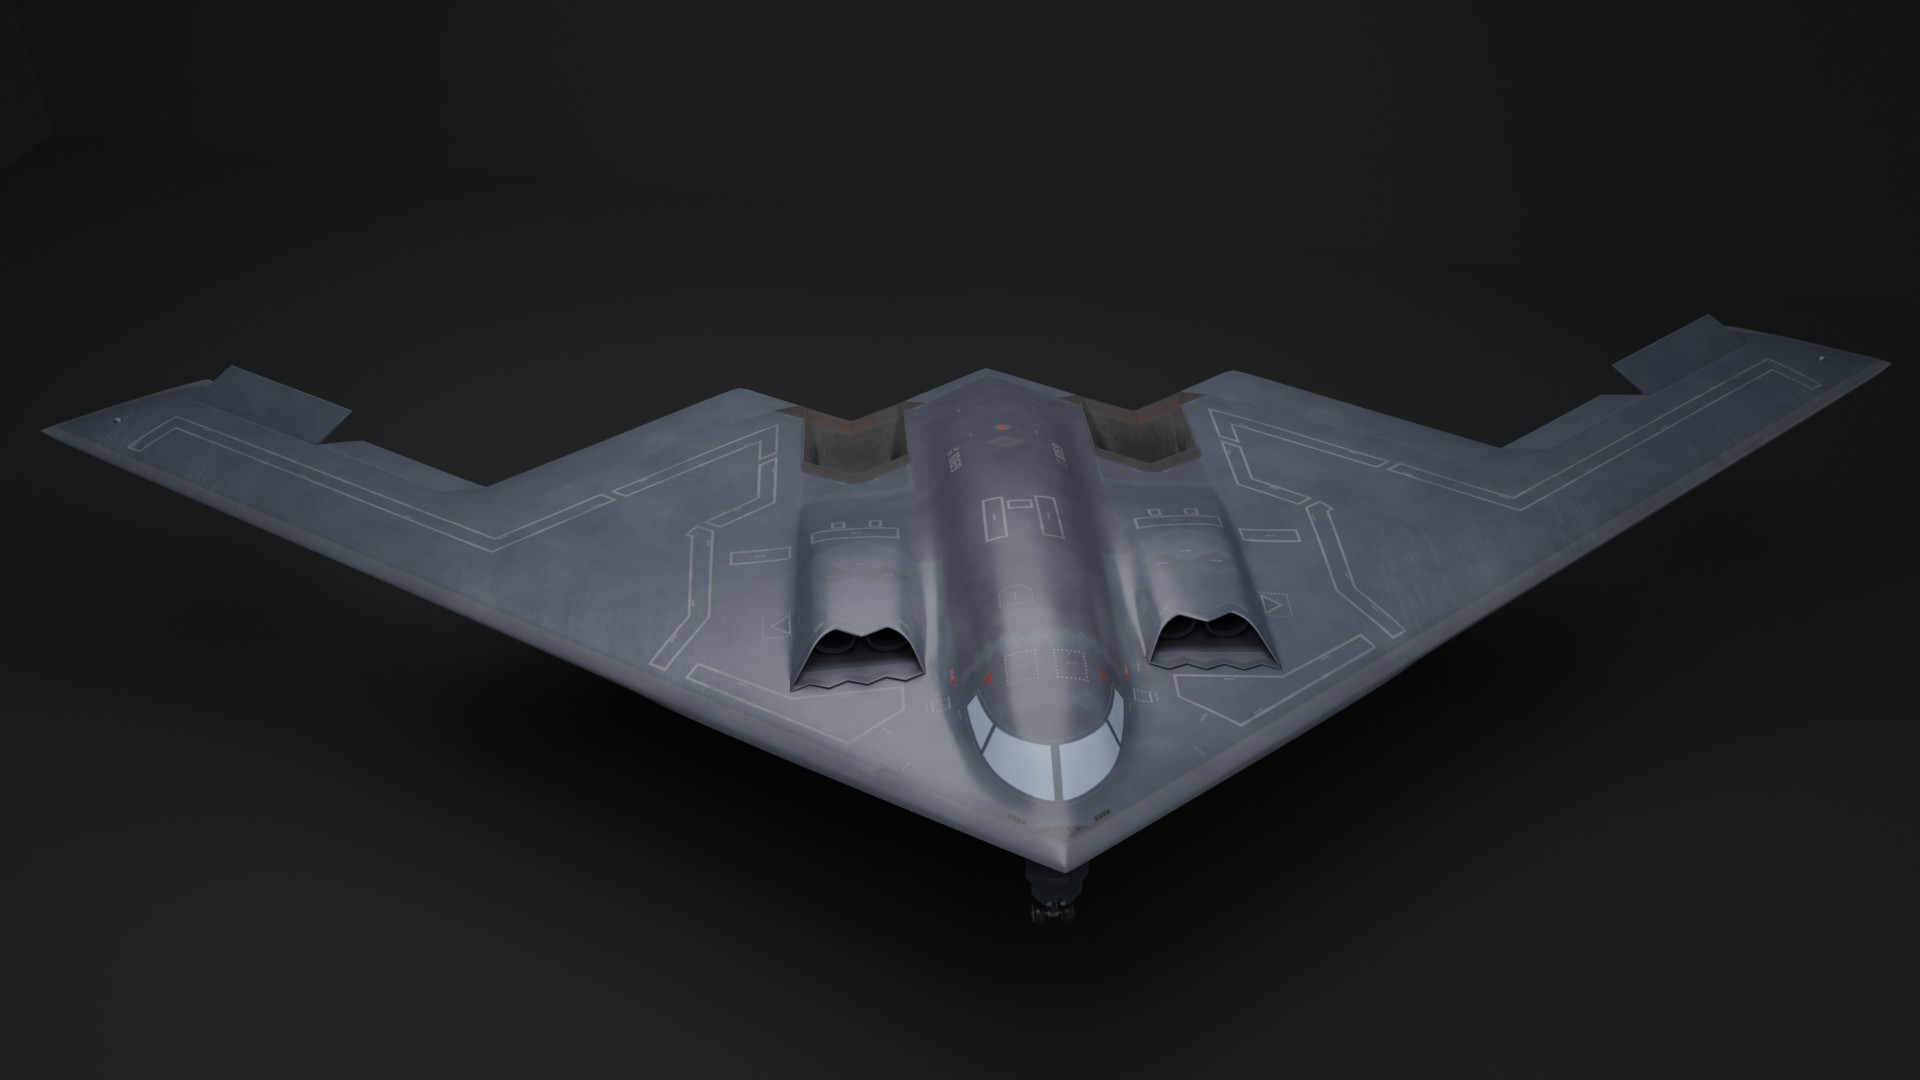
\includegraphics[width=\textwidth]{Code/B2_Model/B-2_Spirit_3D_Model/file-1735478931621.jpg}
        \caption{3D CAD model of the B-2 Spirit aircraft. Taken from~\cite{payne_b2spirit_3d}.}
        \label{fig:3D_model_B2}
    \end{subfigure}
    \hfill
    \begin{subfigure}[b]{0.31\textwidth}
        \centering
        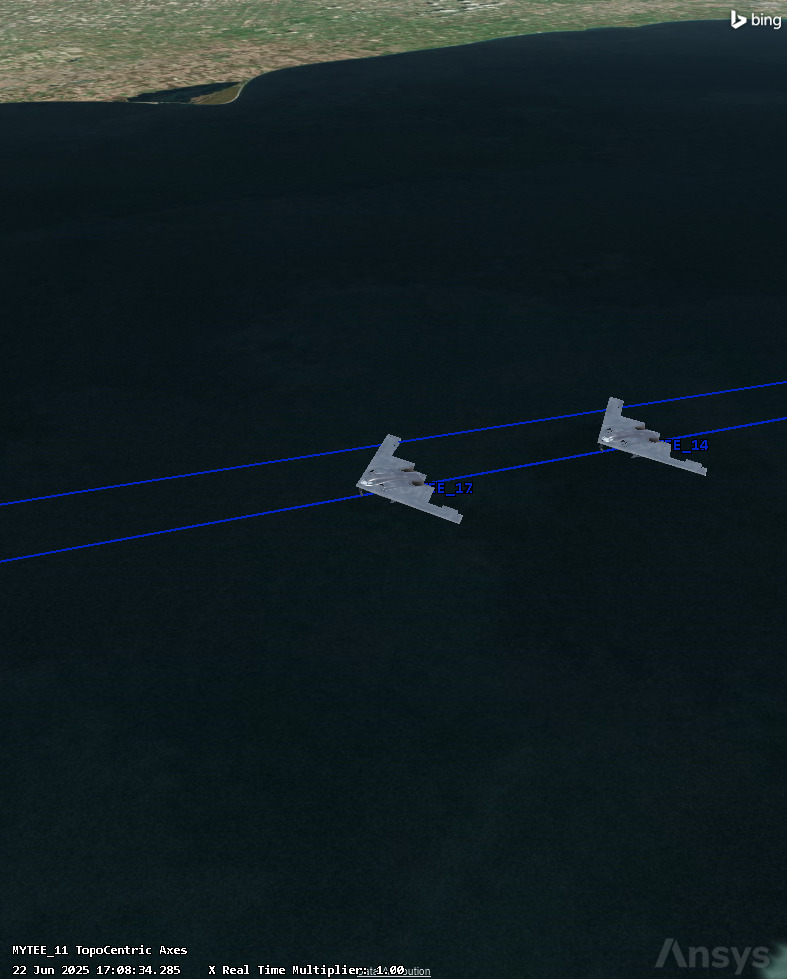
\includegraphics[width=\textwidth]{LaTeX/Figures/B2_Return.jpg.jpg}
        \caption{STK zoomed view.}
        \label{fig:B2_model_in_STK}
    \end{subfigure}
    
\end{figure}

During the mission, a total of 6 refuelling events occurred (3 refuellings per leg). According to~\cite{lemay2025midnight}, the first refuelling operation took place over US soil, the second over the Atlantic Ocean (in international waters), and the third over the Mediterranean Sea (also in international waters), with the precise locations still classified. Information about where the tanker aircraft took off, and their trajectories, is also classified. It was assumed that the outbound leg refuellings occurred over Ohio, the \SI{-30}{\degree} longitude meridian on the great circle trajectory over the Atlantic, and in the waters south of Crete, respectively, and that the return leg refuellings occurred over the same locations, but in reverse. These approximations were informed by unclassified B-2 refuelling locations for Operation Iraqi Freedom (2003) and by the proximity of these locations to US Air Force and Navy bases. In particular, we modelled the tanker aircraft as KC-135 Stratotankers taking off from Wright-Patterson Air Force Base, OH; Lajes Field, located off the coast of Portugal; and Incirlik Air Base in Türkiye, respectively. The facilities created over these bases are shown in Figure~\ref{fig:lajes_field}, Figure~\ref{fig:lajes_field}, and Figure~\ref{fig:lajes_field}, respectively. The precise coordinates of these air force bases were retrieved from the Air Force website at~\cite{ingram_basemap}, and the refuelling operation locations were approximated as those of the Iraqi Freedom mission. The refuelling was modelled using \texttt{Aviator}, with the loiter orbit chosen as a small figure-8 orbit for each aircraft and a speed of \SI{0.05}{\kilo\metre\per\second}. The decoy package of 6 B-2 Spirit bombers was modelled using aircraft STK objects propagated using \texttt{GreatCircle}. Their trajectory was made to follow the reported flight route outlined in Section~\ref{sec:mission_overview}. The support package's takeoff, rendezvous and landing locations, as well as its exact composition, are all classified. Since these aircraft played no relevant active role and had no reported impact on the mission's success, we did not include them in our STK model.

\begin{figure}
    \centering
    \begin{subfigure}[b]{0.32\textwidth}
        \centering
        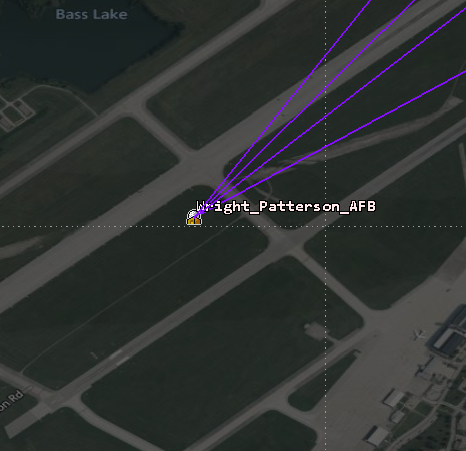
\includegraphics[width=\textwidth]{LaTeX/Figures/WP_AFB.png}
        \caption{W. Patterson AFB.}
        \label{fig:wright_patterson}
    \end{subfigure}
    \hfill
    \begin{subfigure}[b]{0.32\textwidth}
        \centering
        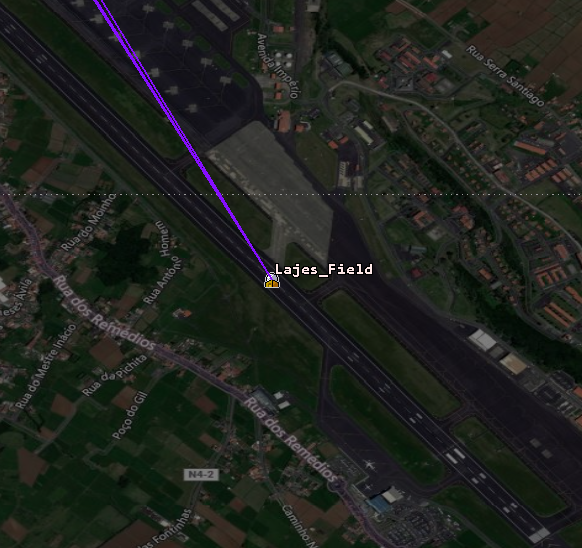
\includegraphics[width=\textwidth]{LaTeX/Figures/Lajes_AFB.png}
        \caption{Lajes Field, Portugal.}
        \label{fig:lajes_field}
    \end{subfigure}
    \hfill
    \begin{subfigure}[b]{0.32\textwidth}
        \centering
        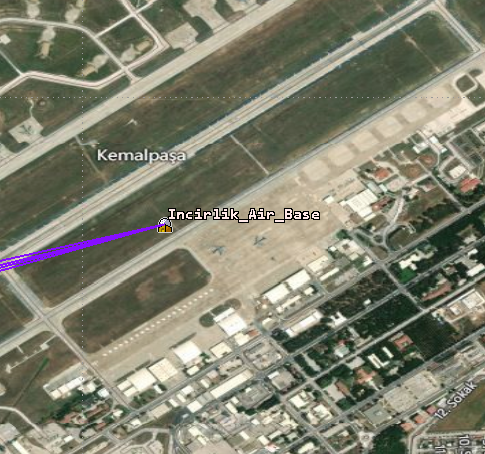
\includegraphics[width=\textwidth]{LaTeX/Figures/Incirlik_AFB.png}
        \caption{Incirlik AFB, Türkiye.}
        \label{fig:incirlik}
    \end{subfigure}

    \label{fig:takeoff_locations}
\end{figure}

\subsection{Maritime forces and Tomahawk missiles}
The attack on Isfahan was carried out remotely by a joint fleet of US and Israeli ships and submarines. The precise identity of the assets used is classified, but both the USS Georgia nuclear submarine and the ISN Rahav Israeli warship were reported to have taken part in the operation. Thus, these are the two maritime forces present in our model. Although the trajectory of these vessels was not disclosed in any of the official reports, we assumed they were jointly deployed in the Persian Gulf and modelled them as ship objects (propagated using \texttt{GreatArc}) in STK. Both vessels reached their target destination off the southern coast of Iran, opening fire at 21:00:00 UTC. A closeup of the USS Georgia model, as well as the trajectory of the Tomahawk missiles it fired on Isfahan (orange trajectory), are shown in Figure~\ref{fig:USS_georgia_model} and Figure~\ref{fig:USS_georgia_firing}, respectively. In this figure, the ISN Rahav ship model is hidden for visibility. The Tomahawk missiles were modelled using the STK missile object, with a ballistic trajectory launching from the warships onto the Isfahan Nuclear Technology Centre and a fixed delta-v of \SI{3.235}{\kilo\metre\per\second}.
\begin{figure}
    \centering
    \begin{subfigure}[b]{0.49\textwidth}
        \centering
        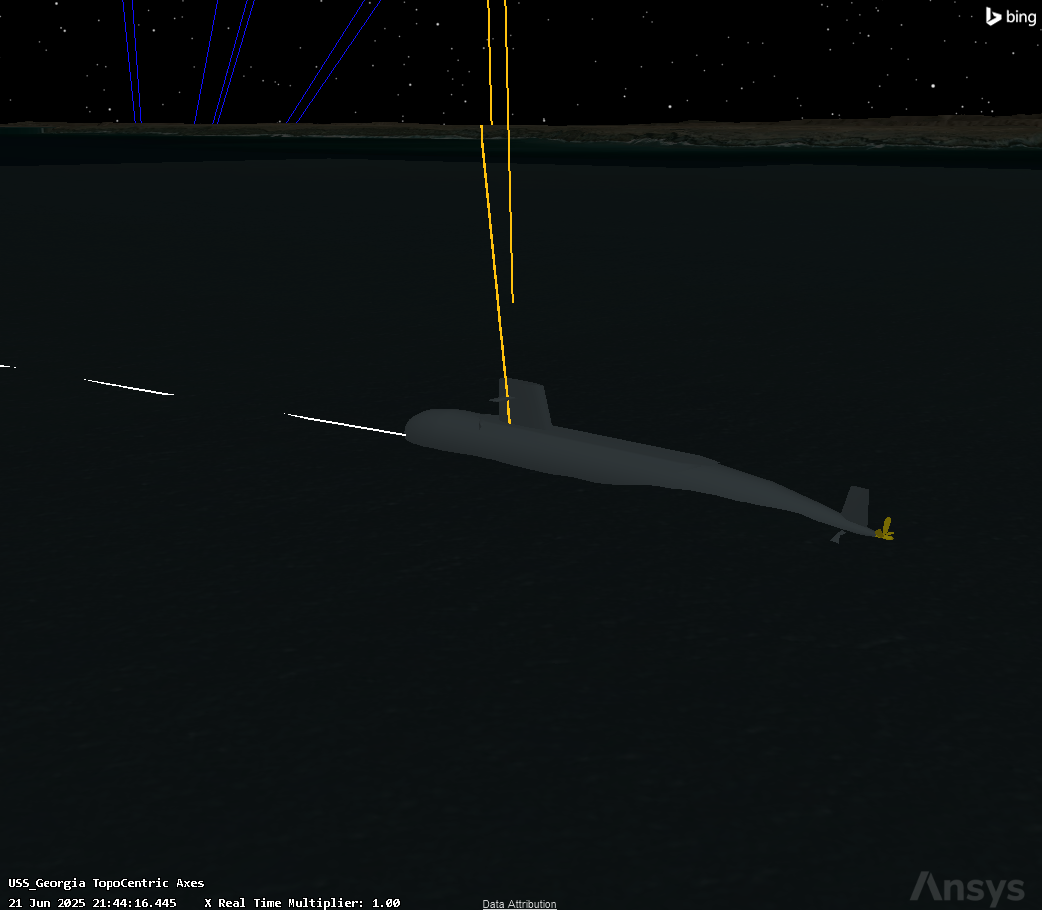
\includegraphics[width=\textwidth]{LaTeX/Figures/USS_Georgia_closeup.png}
        \caption{Closeup of the USS Georgia model.}
        \label{fig:USS_georgia_model}
    \end{subfigure}
    \hfill
    \begin{subfigure}[b]{0.49\textwidth}
        \centering
        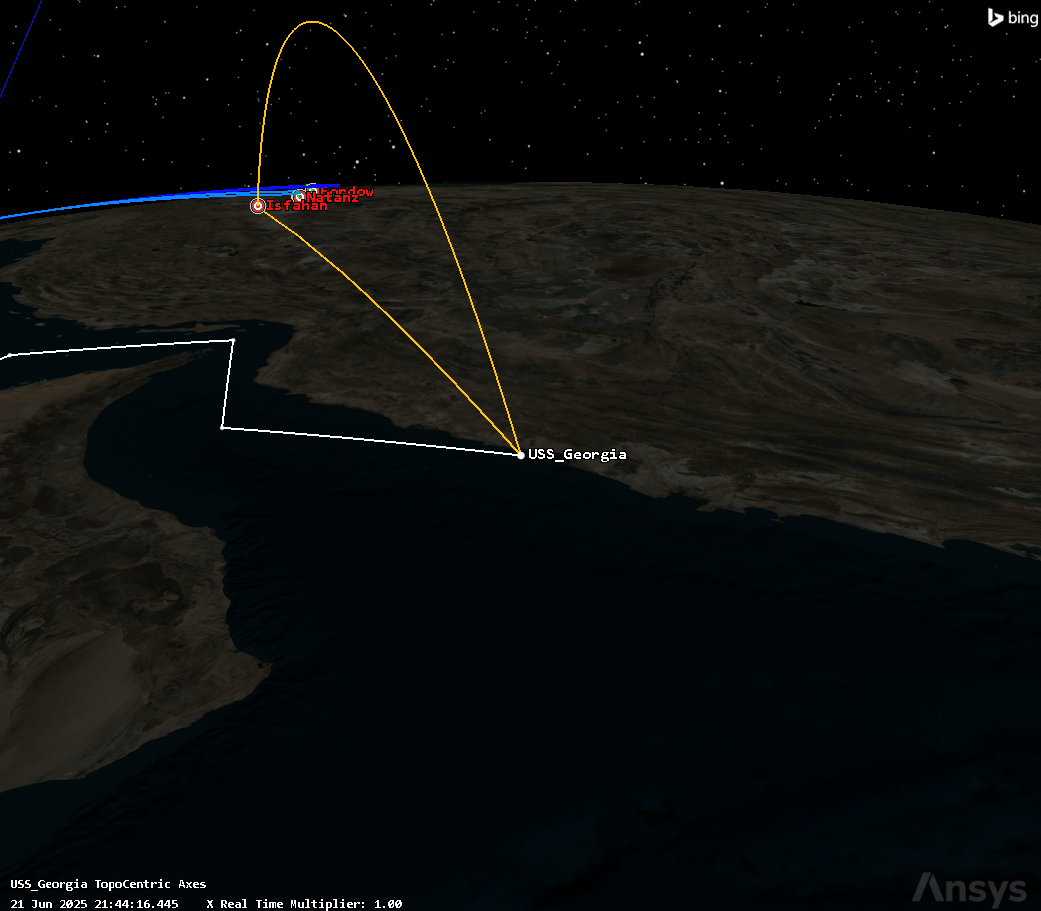
\includegraphics[width=\textwidth]{LaTeX/Figures/USS_Georgia Launch.png}
        \caption{Tomahawks missiles launched on Isfahan.}
        \label{fig:USS_georgia_firing}
    \end{subfigure}
    
\end{figure}

\subsection{GBU-57 bunker buster bombs}
The attacks on Fordow and Natanz were carried out by the main B-2 Spirit package discussed in Section~\ref{subsec:aircraft}. The bombs dropped on these two targets were GBU-57 MOP (also known as ``bunker busters"), \SI{13608}{\kilo\gram} warheads which can penetrate up to \SI{61}{\metre} of reinforced concrete. These bombs are only produced in the United States, and three-quarters of the total US stock was deployed in a single night during OMH (a total of 14 bombs were dropped). One such bomb is shown in Figure~\ref{fig:GBU_57} with human beings for size comparison. We modelled these bombs as air-dropped missile objects in STK, with zero delta-v (since the bombs were dropped rather than launched), and a drop location \SI{12}{\kilo\metre} ahead of their targets (this was calculated using the ballistic trajectory of the GBU-57 bombs, which have a terminal velocity of \SI{317}{\metre\per\second}, and the B-2's cruising speed of \SI{250}{\metre\per\second} and initial altitude of \SI{12}{\kilo\metre}. Using these values, the GBU-57 was estimated to stay in the air for approximately \SI{48}{\second} covering \SI{12}{\kilo\metre} downrange). The trajectories of the 14 bombs released over Fordow and Natanz are shown in Figure~\ref{fig:aerial_strikes} (green). In total, 6 of the 7 B-2s released their warheads over Fordow (their trajectories are shown in dark blue in the figure), while the remaining bomber released its two bombs over Natanz (light blue). All times for release and manoeuvres were modelled to exactly match the real mission, discussed in detail in Section~\ref{sec:mission_overview}. 

\begin{figure}
    \centering
    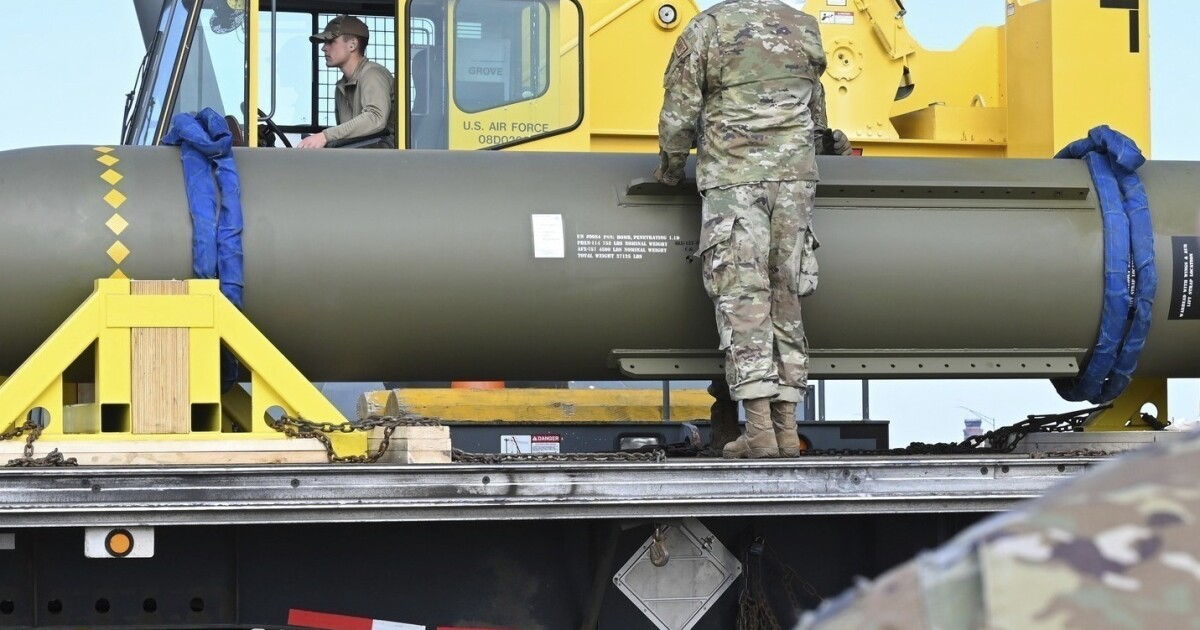
\includegraphics[width=\linewidth]{LaTeX/Figures/GBU_57.jpeg}
    \caption{GBU-57 MOP bomb being transported. The bomb measures \SI{6}{\metre} in length. ABC News.}
    \label{fig:GBU_57}
\end{figure}

\begin{figure}[h]
    \centering
    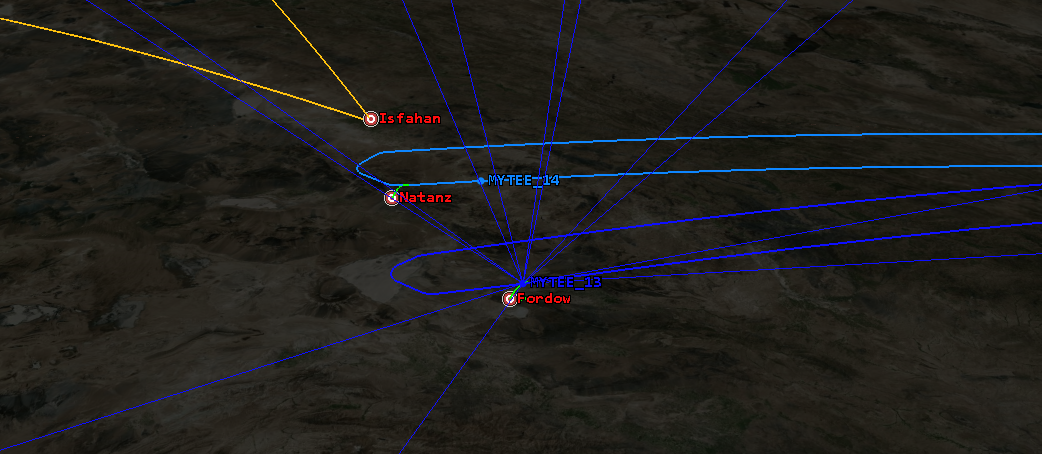
\includegraphics[width=\linewidth]{LaTeX/Figures/aerial_strikes.png}
    \caption{Aerial strike trajectories of GBU-57 MOP bombs dropped from B-2 spirit bombers.}
    \label{fig:aerial_strikes}
\end{figure}

\subsection{Satellites and intelligence}
As discussed in Section~\ref{sec:intro}, satellite intelligence represented the central coordinating element in this mission. We employed a total of 32 satellites to enable lightspeed communication among the several aircraft involved, to track and guide all bombs and missiles, and to support BDA imaging of the sites post-strike. 

\begin{figure}[h]
    \centering
    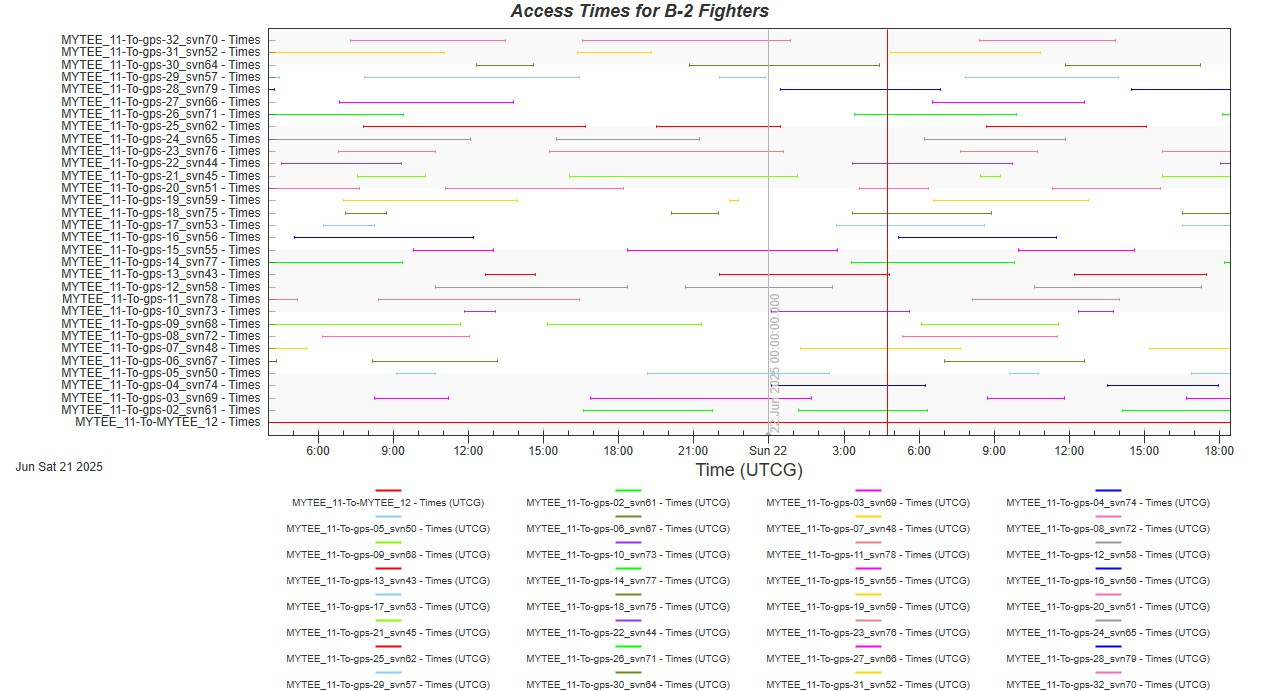
\includegraphics[width=\linewidth]{LaTeX/Figures/Access_B2_Spirit.jpg}
    \caption{Access times for the lead B-2 spirit bomber (codename MYTEE-11) to the GPS constellation.}
    \label{fig:spirit_to_gps}
\end{figure}

To coordinate the missile strikes between the B-2 bombers and the USS Georgia and the ISN Rahav maritime forces, we employed the SBRIS constellation in STK, which granted continuous access between the two forces throughout all mission-critical phases. The route of the B-2 bombers was also continuously tracked using the GPS constellation: access times between the lead bomber and GPS satellites are shown to give continuous coverage in Figure~\ref{fig:spirit_to_gps}. This enables the onboard positioning and guidance system to provide continuous corrections to the route of the B2 bombers, enabling them to follow the predetermined mission path. In addition, GPS positioning is crucial for the coordination of refuelling maneuvers, which demand the KC-135 Stratotankers to approach the B2 bombers with incredibly accurate matching of both position and velocity, to accurately dock the fuel pipe into the stealth aircraft's conduit. The communication access prior to the third outbound refuelling maneuver is displayed in Figure~\ref{fig:access_refuel} to showcase the centrality of space intelligence throughout this mission phase.

\begin{figure}[h]
    \centering
    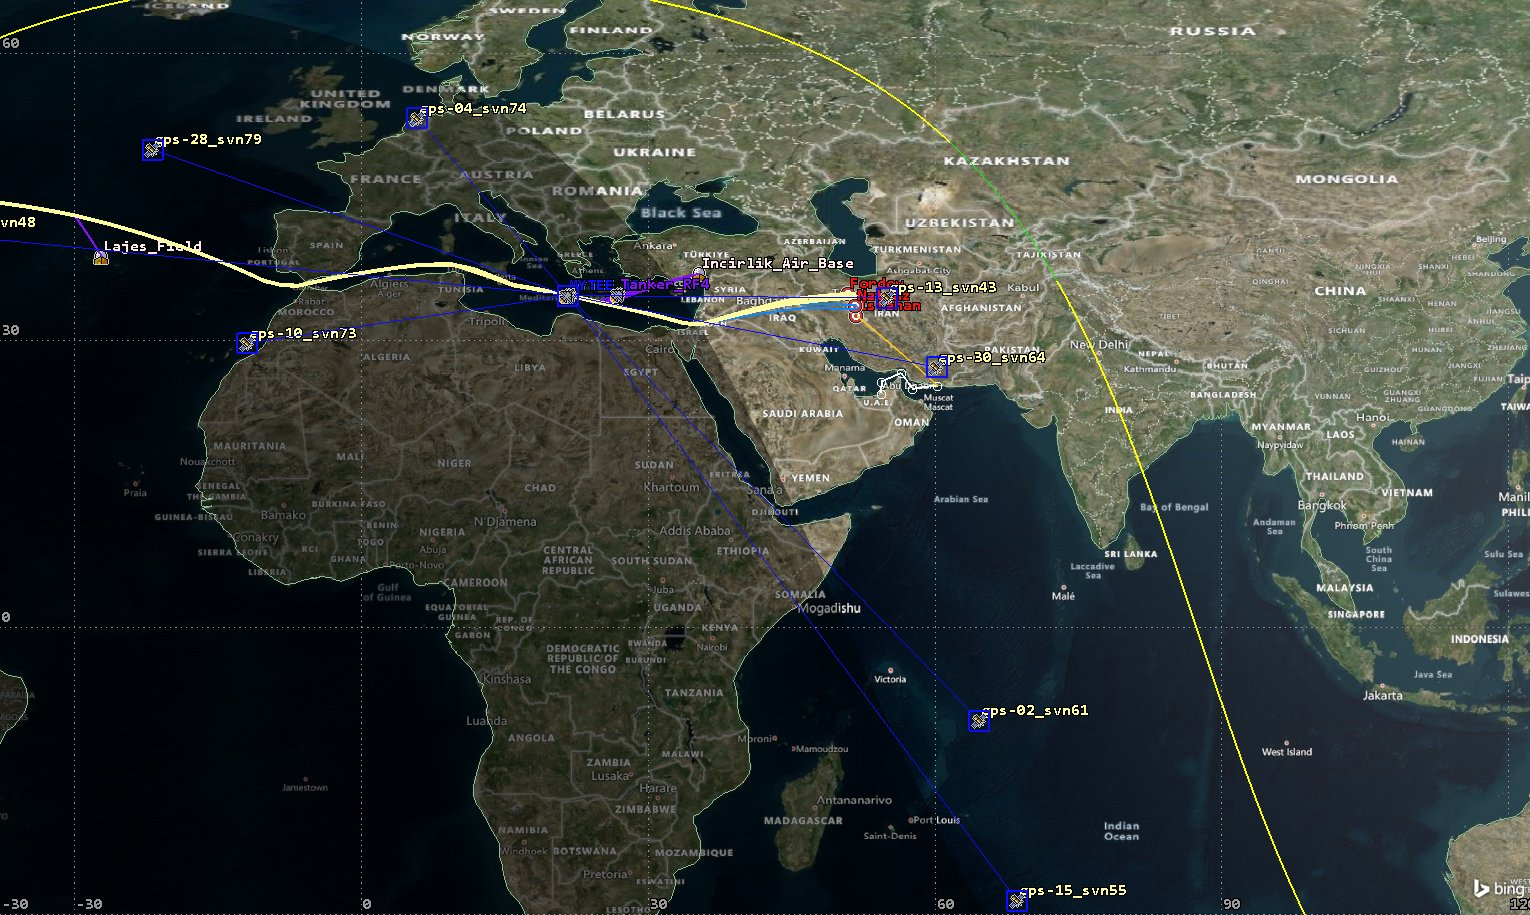
\includegraphics[width=\linewidth]{LaTeX/Figures/Access_Graphic_Pre_Refuelling.jpg}
    \caption{Acess status immediately prior to the initiation of the third refuelling maneuver (over the Mediterranean Sea).}
    \label{fig:access_refuel}
\end{figure}

Further, the GPS constellation was used to guide the GBU-57 bombs and the Tomahawk missiles. These warheads have very narrow mission durations, and their access times are shown in Figure~\ref{fig:gbu_57_access} and Figure~\ref{fig:tomahawk_access}, respectively. Although brief, these communication windows were essential to the success of the mission: the Tomahawk missiles have an active control system which guided all 75 units to their intended target on the surface of Isfahan. Similarly, the GBU-57 bombs have a passive, GPS-enabled grid-fin control system used to correct the course of the warheads to their exact impact location. BDA imaging (discussed in greater detail later) confirmed that, out of 14 released MOPs, all 14 hit their pre-determined coordinates with an error below \SI{5}{\metre}. This unforseen degree of precision is entirely enabled by space intelligence, and is unprecedented in military history.

\begin{figure}[h]
    \centering
    \begin{subfigure}[b]{0.49\textwidth}
        \centering
        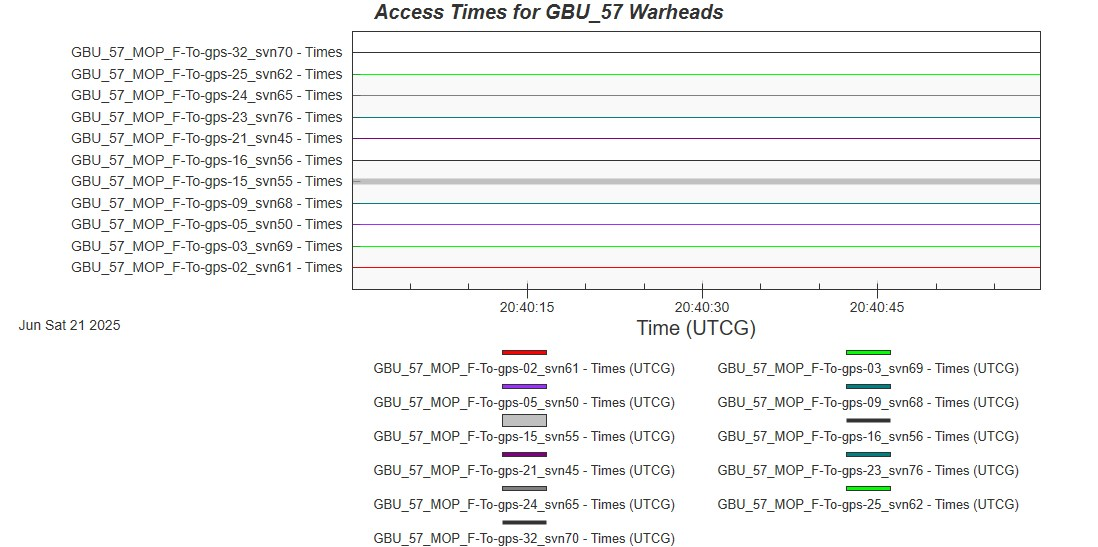
\includegraphics[width=\textwidth]{LaTeX/Figures/Access_GBU_57.jpg}
        \caption{Access times for GBU-57 bomb.}
        \label{fig:gbu_57_access}
    \end{subfigure}
    \hfill
    \begin{subfigure}[b]{0.49\textwidth}
        \centering
        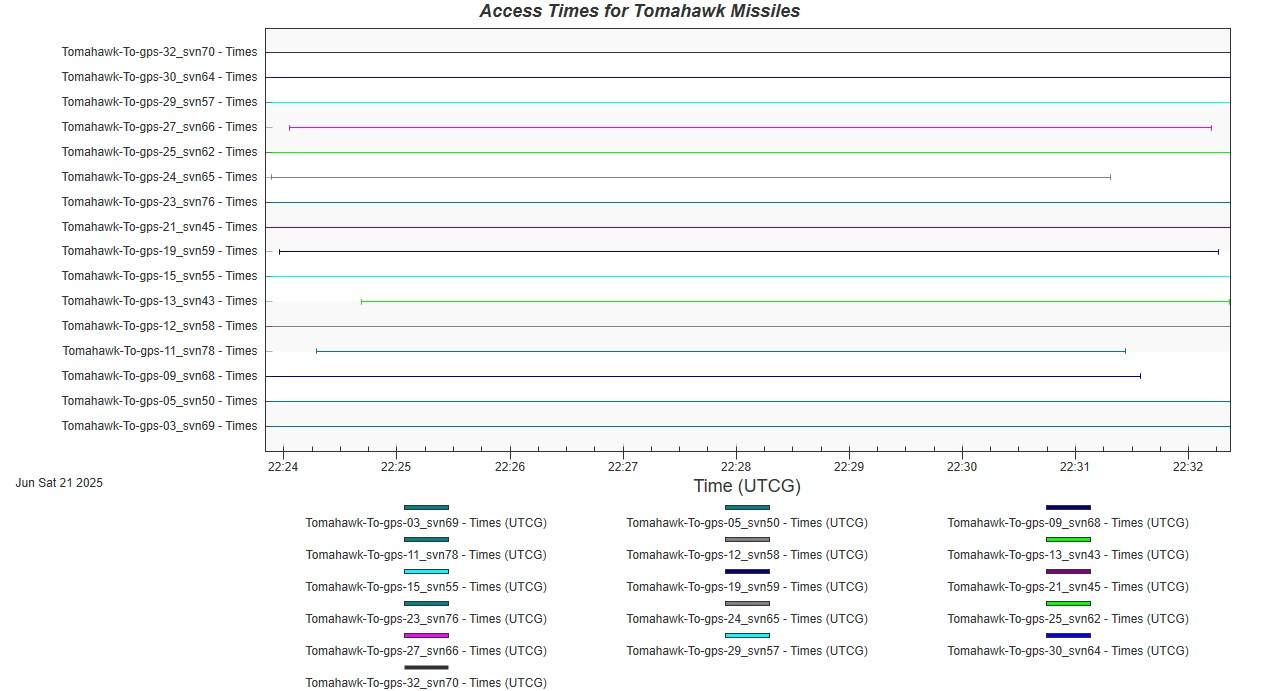
\includegraphics[width=\textwidth]{LaTeX/Figures/Access_Tomahawk.jpg}
        \caption{Access times for Tomahawk missile.}
        \label{fig:tomahawk_access}
    \end{subfigure}
    
\end{figure}

For BDA imaging, the documentation available as of the writing of this report does not include any details about the exact satellites used in OMH. However, there is no doubt that some low-earth orbit (LEO) electro-optical satellite was employed to image the strike locations both before and after impact (we later show the satellite images reported by several news outlets). As a result, we approximated this mission phase, employing a LEO orbit satellite with custom orbital parameters selected to provide two overhead passes before and after the strikes in the daylight (altitude \SI{500}{\kilo\metre}, inclination \SI{67.7053}{\degree}, RAAN \SI{224}{\degree} and other parameters zero at the starting epoch). These passes are shown in Figure~\ref{fig:pre_strike} and Figure~\ref{fig:post_strike}, respectively. The satellite was also equipped with a downward-facing sensor with conical field of view and a view angle of \SI{45}{\degree} to simulate the onboard camera. Using this sensor, we were able to compute the visibility of the targets throughout the overhead passes. Through a process of iterative refinement, we were eventually able to refine the orbital elements so to guarantee visibility with the two overhead passes, to provide imaging both before and after the strikes. The coverage provided by the chosen LEO electro-optical satellite over the three nuclear facilities is shown in Figure~\ref{fig:satellite_coverage}.

\begin{figure}[h]
    \centering
    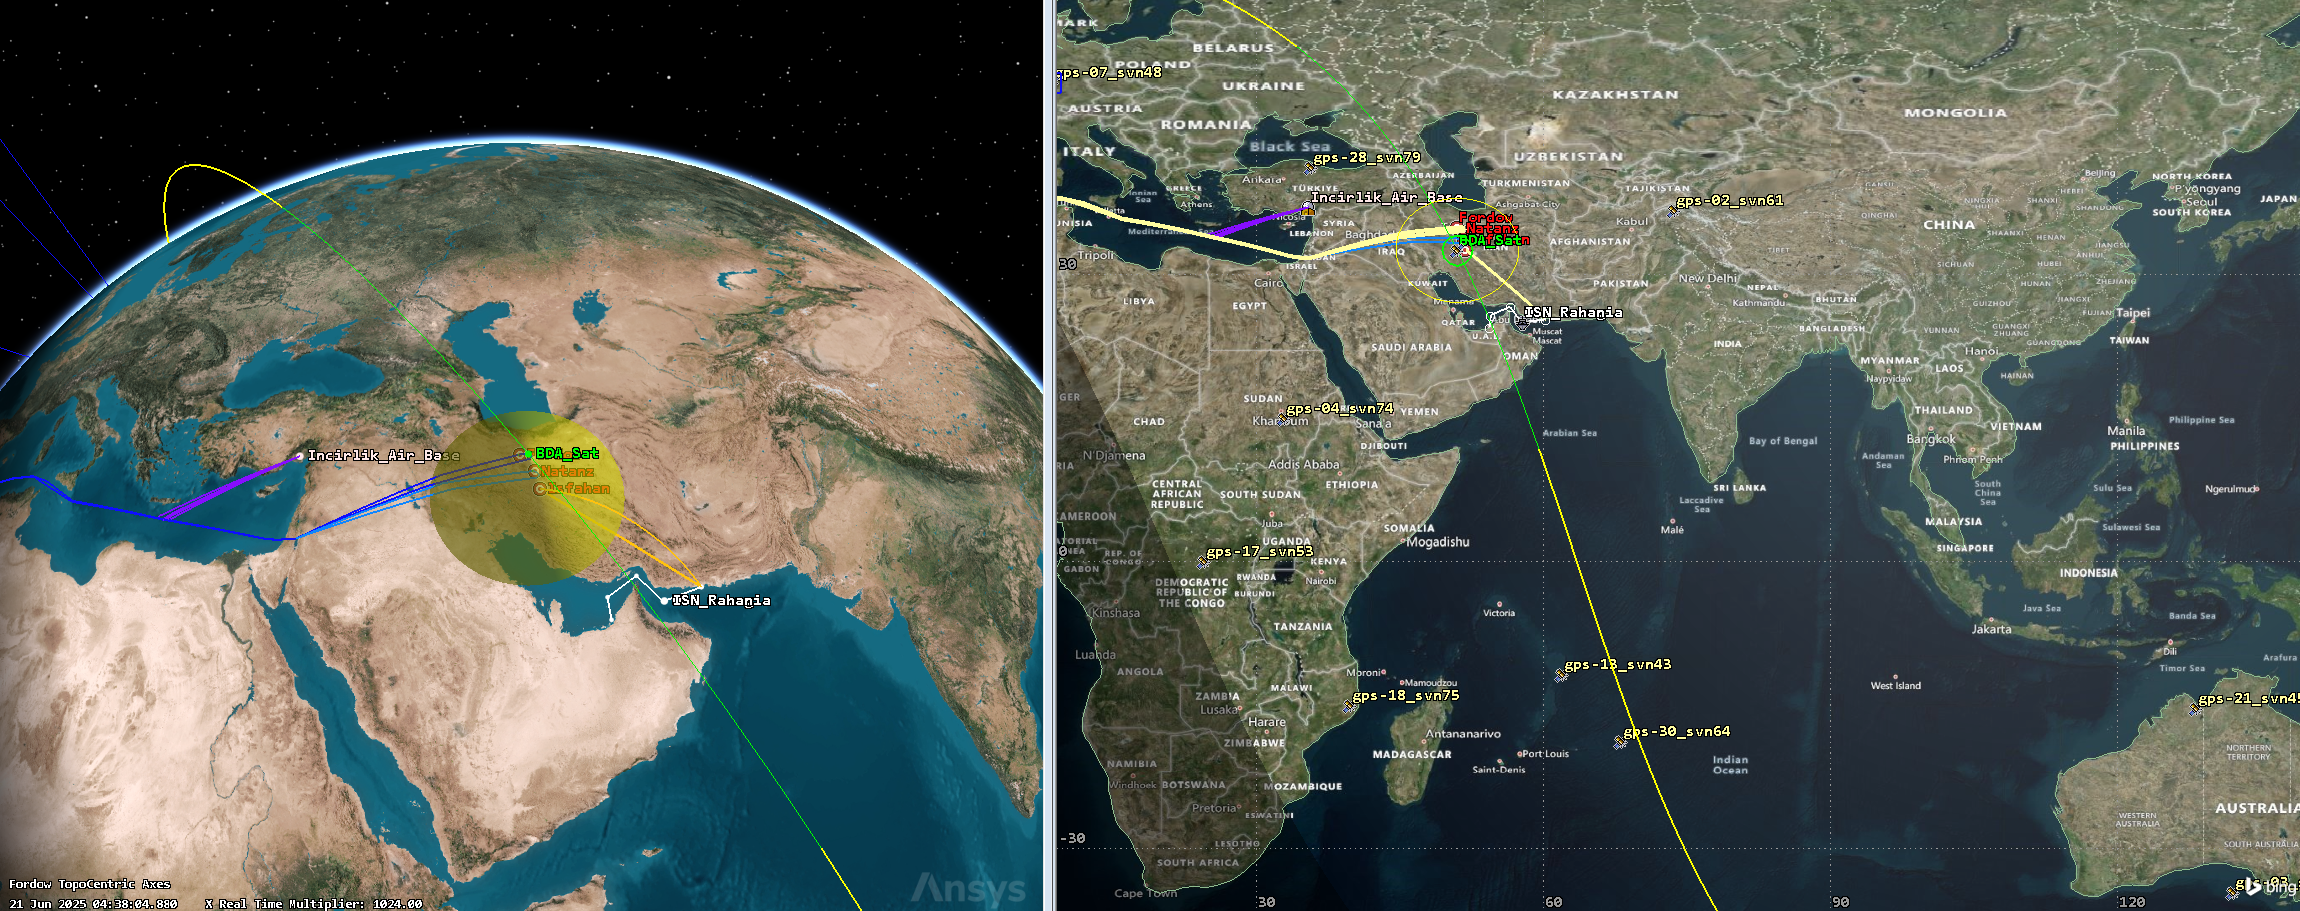
\includegraphics[width=\linewidth]{LaTeX/Figures/Pre_strike_assessment.png}
    \caption{Pre-strike imaging by the LEO electro-optical satellite.}
    \label{fig:pre_strike}
\end{figure}


\begin{figure}
    \centering
    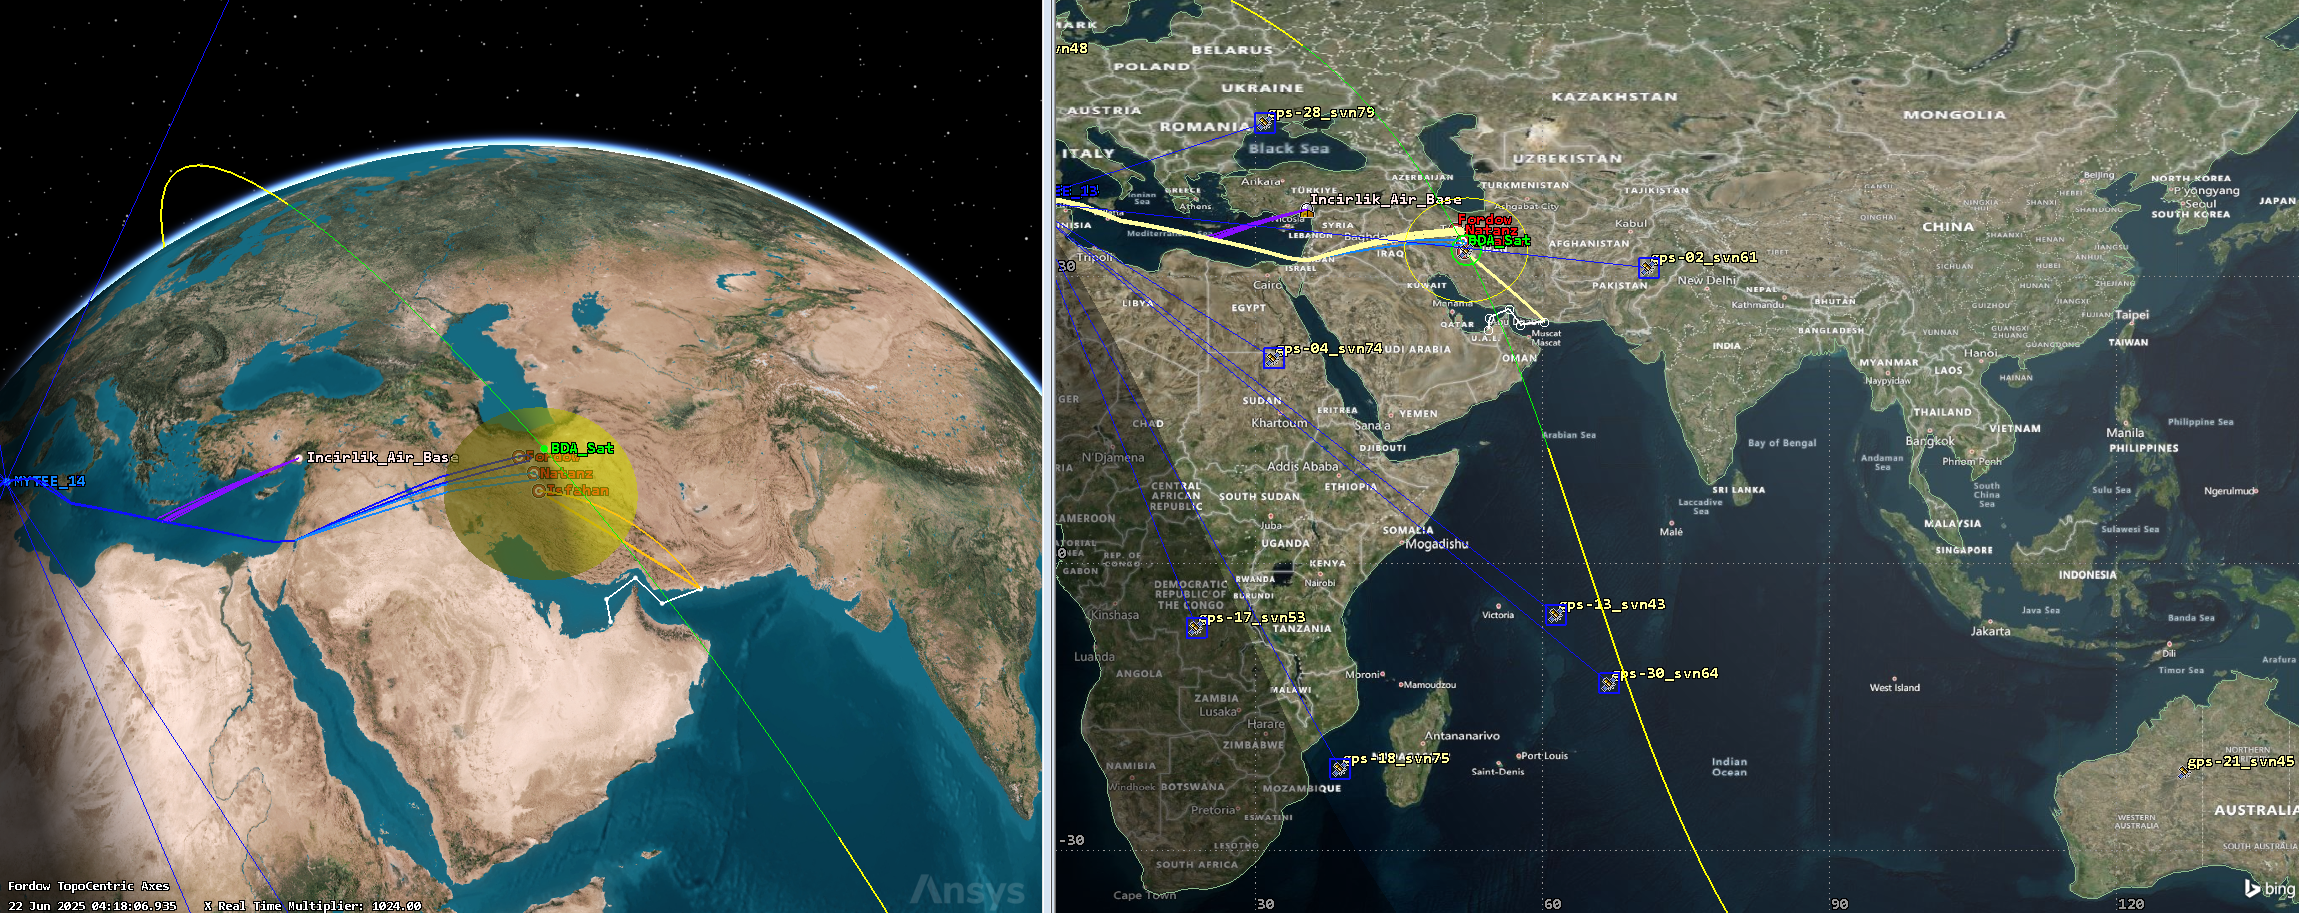
\includegraphics[width=\linewidth]{LaTeX/Figures/Post_Strike_assessment.png}
    \caption{Post-strike imaging by the LEO electro-optical satellite.}
    \label{fig:post_strike}
\end{figure}

\begin{figure}
    \centering
    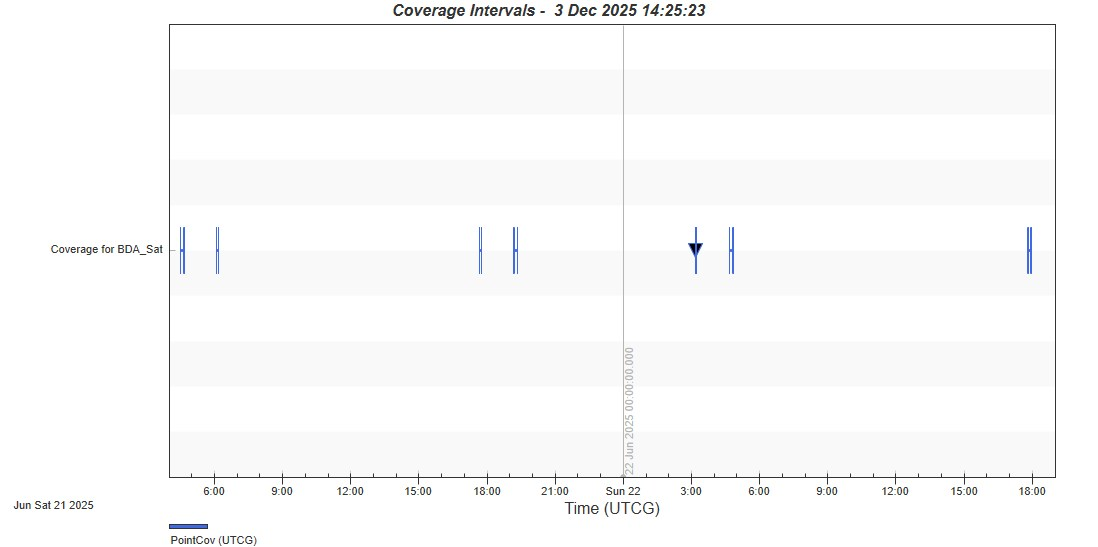
\includegraphics[width=\linewidth]{LaTeX/Figures/Coverage_for_BDA_Sat.jpg}
    \caption{STK coverage graph for the LEO electro-optical satellite over the three facilities.}
    \label{fig:satellite_coverage}
\end{figure}

Finally, true images captured by the real satellite (here modelled approximately in STK) of the Fordow facility before and after the strikes are shown in Figure~\ref{fig:placeholder}.

This section has highlighted the importance of space intelligence in modern military missions. In the accompanying video, we demonstrate the STK implementation of our model. In particular, we want to ask the viewers to notice the two overhead passes of the LEO electro-optical satellite over the three target facilities, noticing how they occur as soon as the sun rises over the locations. We also want to highlight the access computations, visible throughout the mission, between the bombers, bombs, missiles, ships and facilities with all employed space intelligence. In particular, in the video we provide a sample of these access computations by zooming close to the Tomahawk missiles right before they are launched, and following their trajectory as they rise over the horizon and head towards their final targets. In this sequence, the connections between missile and constellations are made explicitly visible. We note that, for every other mission-critical communication phase, we employed a similar level of analysis to ensure guaranteed access between the various mission units. This was done in order to increase the fidelity of our model to the real-world mission.

\begin{figure}
    \centering
    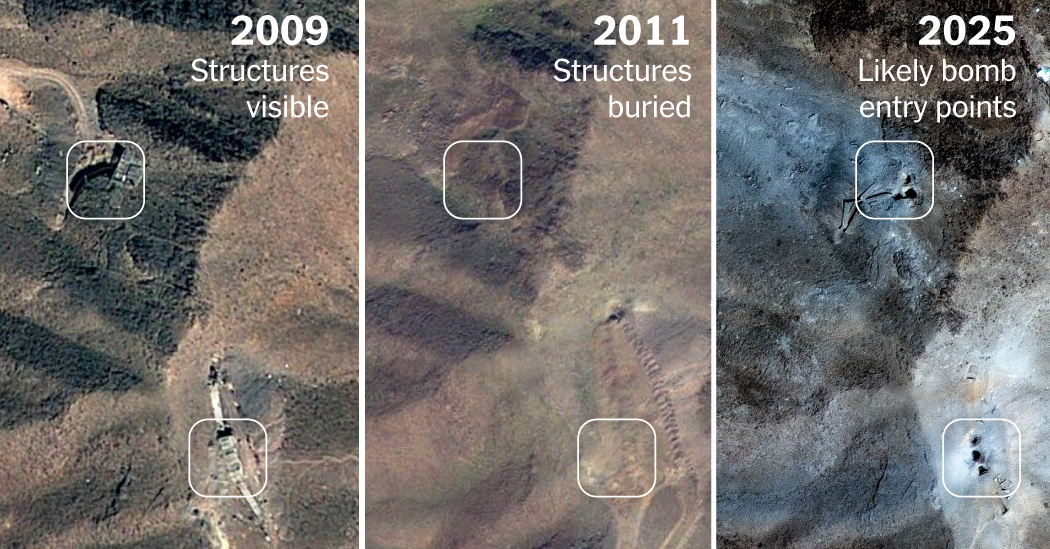
\includegraphics[width=\linewidth]{LaTeX/Figures/2025-06-22-fordo-before-after-ventilation-shafts-index-facebookJumbo-v3.jpg}
    \caption{Post-strike BDA images over Fordow. Credit: New York Times.}
    \label{fig:placeholder}
\end{figure}


\ifpartB
\section{Expansion: HammerEye}

\subsection{Purpose}
The purpose of this extension is to build on the replication of Operation Midnight Hammer in Part A and enhance the mission through space-based assets. Out mission expansion introduces a new spy satellite constellation: \textbf{HammerEye}. This constellation augments the original mission by creating surveillance infrastructure to monitor the activity around the three nuclear facilities after the strikes. This is done to observe any attempts at reconstruction and/or the transportation of key resources to other facilities by the Iranian military. This space surveillance system extends the original objectives of OMH to not only set back the Iranian nuclear program by a few years, but also to guarantee a long period of stability and prevent escalations, extending the original mission objective by several years into the future.

\subsection{Goals and Objectives}
The expanded goal is to strengthen the effectiveness of Operation Midnight Hammer by adding a space-based surveillance phase. This phase aims to monitor the targeted Iranian nuclear sites for signs of reconstruction or retaliatory actions, turning the mission from a short-term strike into a longer-term deterrence strategy. The mission type is a combination of intelligence gathering and technology demonstration. This extension brought the total object count in our STK model to over 100.

Measurable objectives include achieving at least 50 per cent daylight coverage over the three key sites in Iran, with average revisit times of less than 50 minutes to allow for near-real-time detection of activities.

\subsection{STK Mission Design}
In this extension, the spacecraft system consists of a small constellation of fifteen LEO satellites, using a combination of 5 direct optical imaging satellites and 10 infrared detection satellites. Each satellite is equipped with imaging sensors and communication tools to monitor the sites and relay data. This setup solves the problem of limited post-strike intelligence in the original operation, where ground-based or aerial reconnaissance could be risky due to Iranian defences. By using space-based assets, the extension provides persistent, safe oversight that can detect changes like new construction or missile movements.

\subsubsection{Area Target}
To begin the implementation of the HammerEye constellation, we created an \texttt{Area Target}
object. This object was created using an AreaType of ``Pattern", and the Iran\_Islamic\_Republic was selected as the target from STK's native list of countries. Figure~\ref{fig:area_target} shows this STK object in the User Window from a TopoCentric Axes view zoomed to the object. This object represents the fundamental building block to contruct the coverage definition discussed in the following subsection.

\begin{figure}[h]
    \centering
    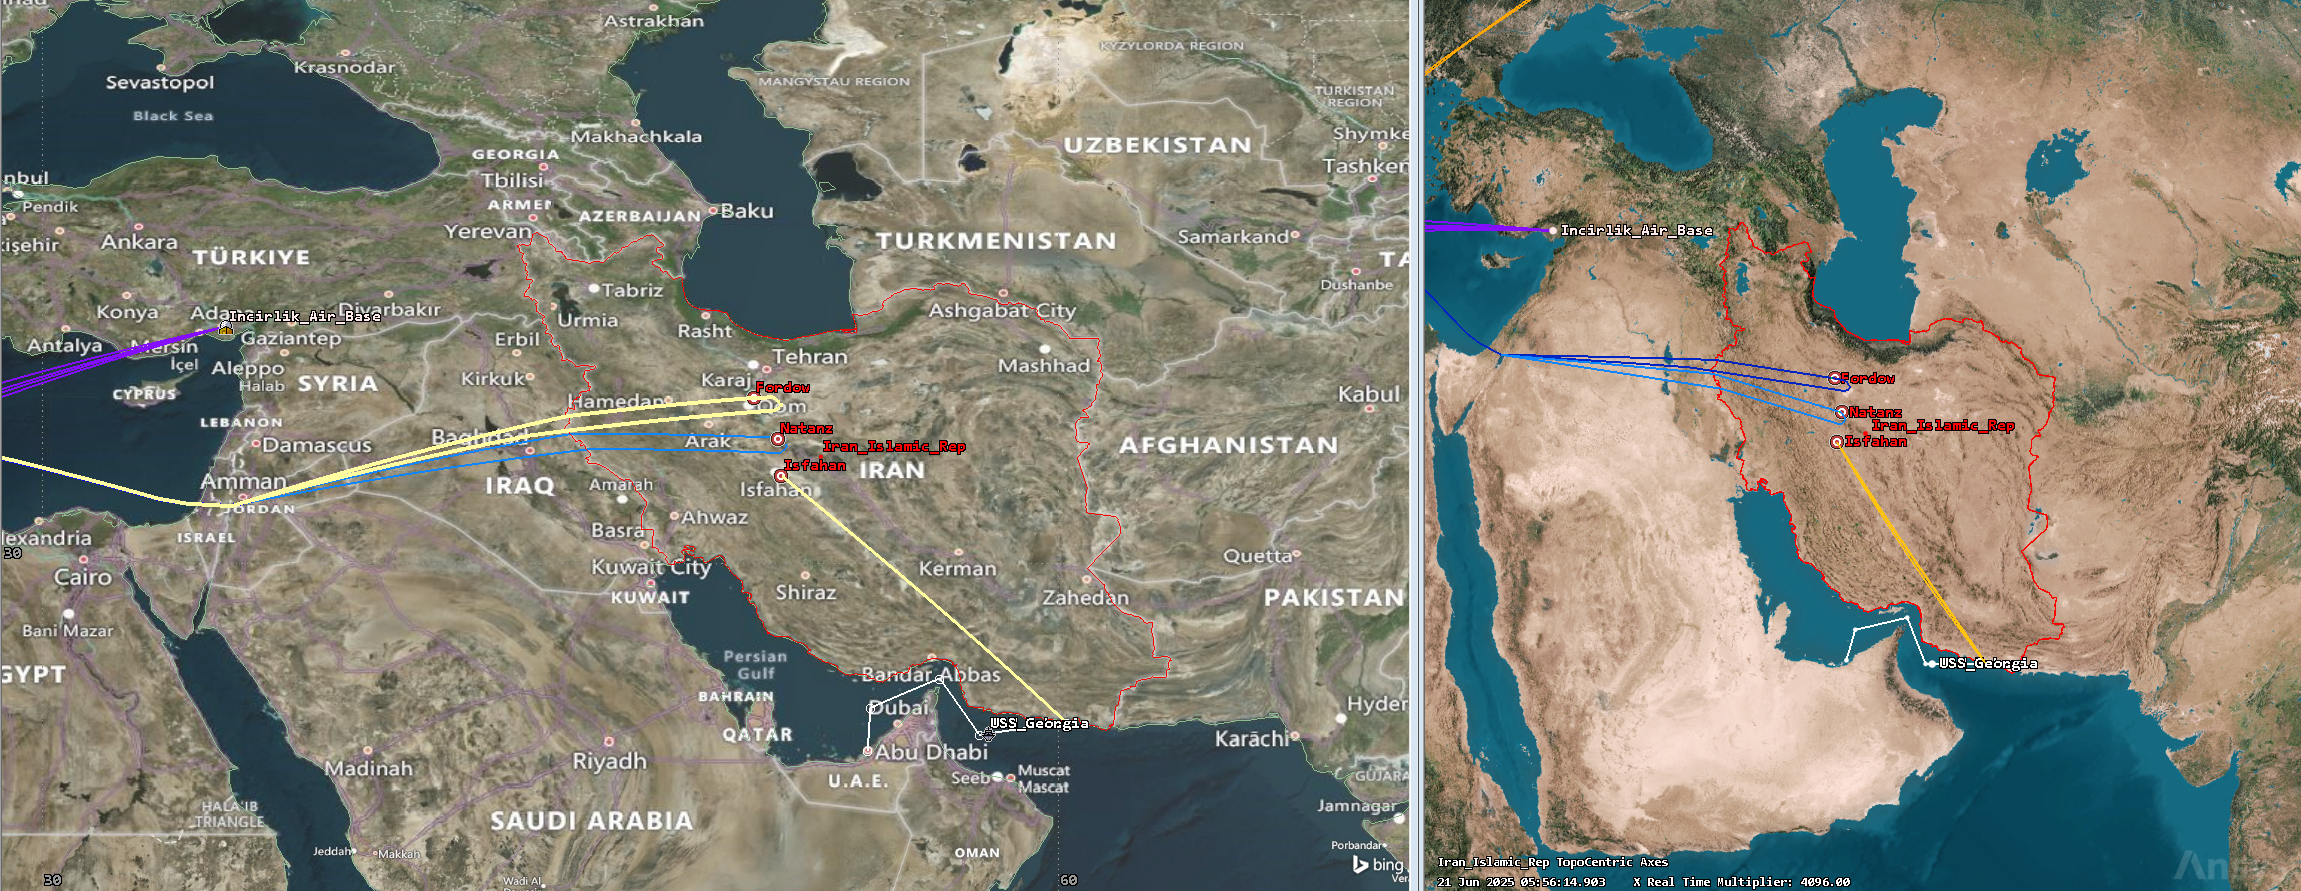
\includegraphics[width=\linewidth]{LaTeX/Figures/AreaTarget.png}
    \caption{2D (left) and 3D (right) STK windows of the AreaTarget object (red outline) over the country of Iran. Facility targets are also visible.}
    \label{fig:area_target}
\end{figure}

\subsubsection{Coverage Definition}
Next, we created a \texttt{CoverageDefinition} STK object to model the surveillance access windows over Iran. In the Grid Area of Interest window, we selected the Area Target object described in the previous subsection. To enhance the resolution of this coverage, in the Point Definition window we enhanced the ``Grid Granularity" to a Latitude/Longitude grid resolution of \SI{1}{\degree}.

This choice was inspired by the tradeoff of computational complexity with accurate modelling, and we did not refine the resolution further since our principal areas of interest were inland and not on Iran's border (the square approximation is very good in the centre of a country, but starts to show its limitations on the borders).

This coverage definition is displayed in Figure~\ref{fig:coveragedeginition}, where we can see the \SI{1}{\degree} squares tessellating the country of Iran. This coverage definition is used to compute the HammerEye surveillance effectiveness by monitoring which parts of the country of Iran are accessed throughout the day. We note that we did not restrict ourselves to an area surrounding the strike locations, since, in case of a suspicious transportation of nuclear material to other cities, we wanted to ensure our HammerEye surveillance system could capture any movement to any location, however remote.

This definition enabled the computation of coverage and access times to the region, essential for the evaluationg of HammerEye's surveillance capabilities over the country.

\begin{figure}
    \centering
    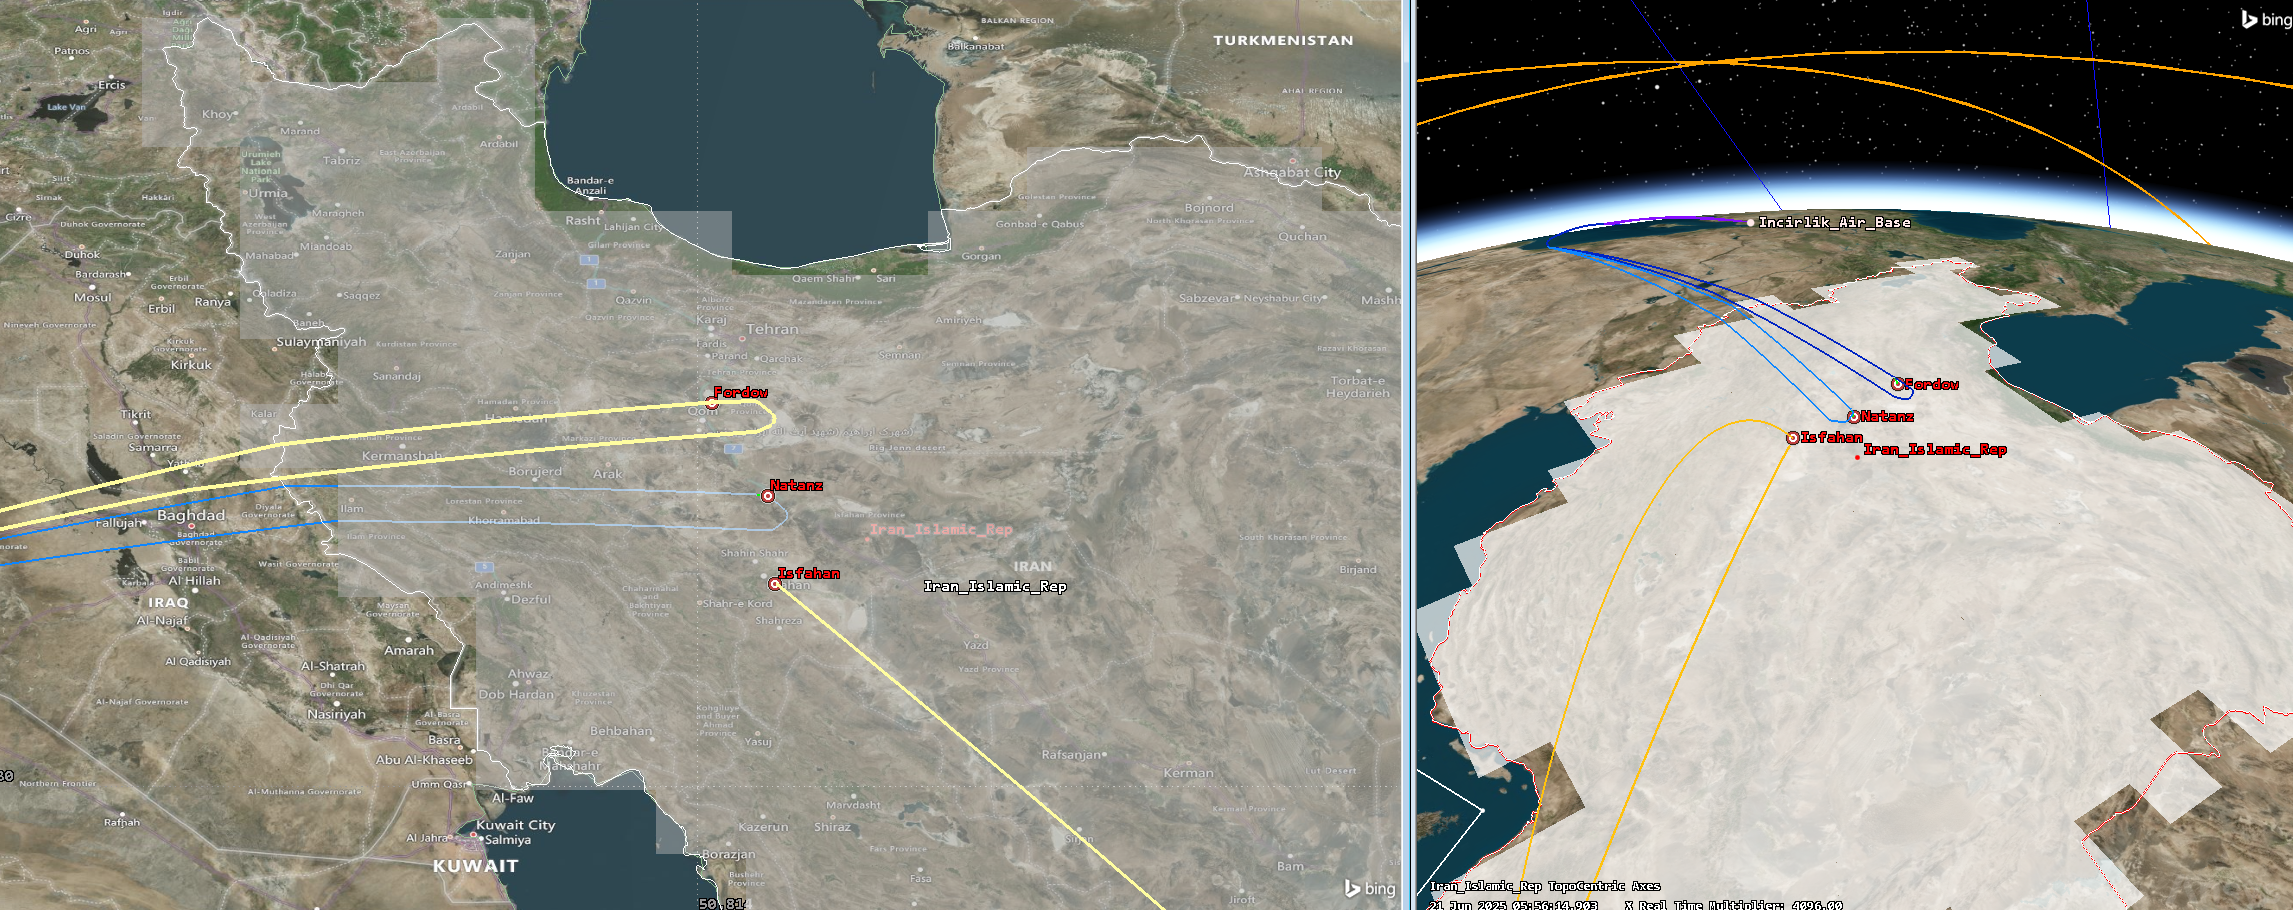
\includegraphics[width=\linewidth]{LaTeX/Figures/CoverageDefinition.png}
    \caption{Coverage definition over Iran. 2D (left) and 3D (right) STK windows. The individual squares making up our topological coverage are clearly visible.}
    \label{fig:coveragedeginition}
\end{figure}

\subsubsection{Optical Satellites}

To model the optical imaging satellites, we generated 5 satellite objects and modelled their orbits using the \texttt{Repeating Ground Track} generator in Orbit Wizard. We selected an altitude of \SI{500}{\kilo\metre} and inclinations of \SI{67}{\degree} for each satellite to ensure proximity to the sites and mitigation of the precession of the line of nodes effect. Each satellite was equipped with a camera sensor with a field of view of \SI{45}{\degree} to guarantee coverage and enable high-resolution imaging. The remaining orbital elements of these satellites were individually selected to ensure the ground tracks would intersect the three nuclear facilities with subsequent passes. All satellites were propagated using HPOP starting on June 21st at 23:00:00 UTC (one hour after the strikes). The launch procedure for these satellites was not modelled as it was deemed outside the scope of this course. Figure~\ref{fig:2d_spysat} and Figure~\ref{fig:3d_spysat} show a snapshot of an overhead pass made by these optical HammerEye satellites.

\begin{figure}[h]
    \centering
    \begin{subfigure}[b]{0.49\textwidth}
        \centering
        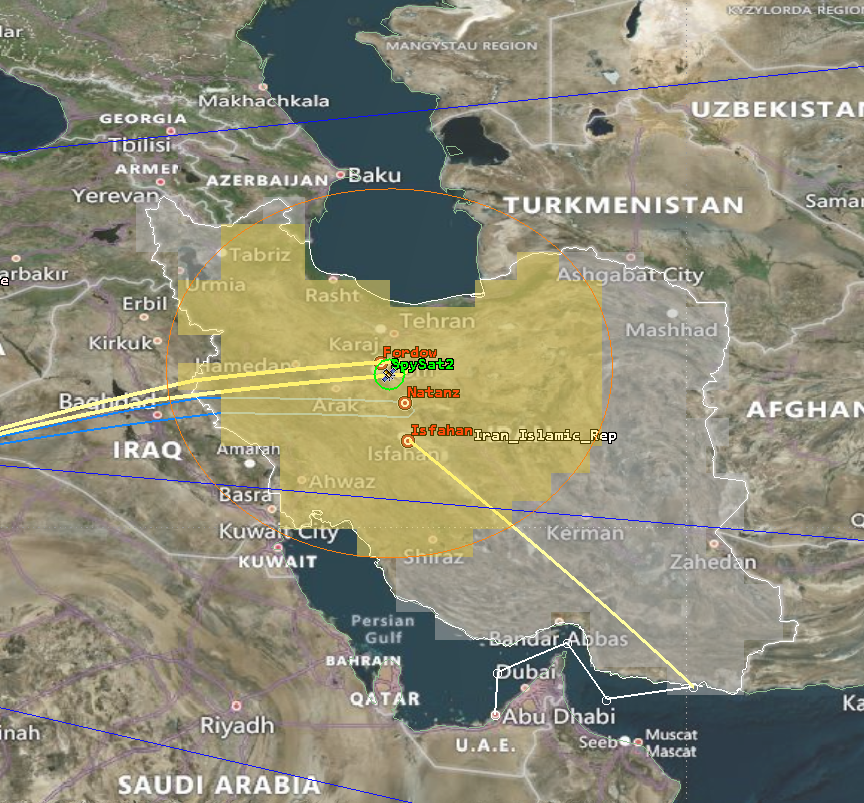
\includegraphics[width=\textwidth]{LaTeX/Figures/OpticalSpy2D.png}
        \caption{3D graphic window of optical spysat pass.}
        \label{fig:2d_spysat}
    \end{subfigure}
    \hfill
    \begin{subfigure}[b]{0.49\textwidth}
        \centering
        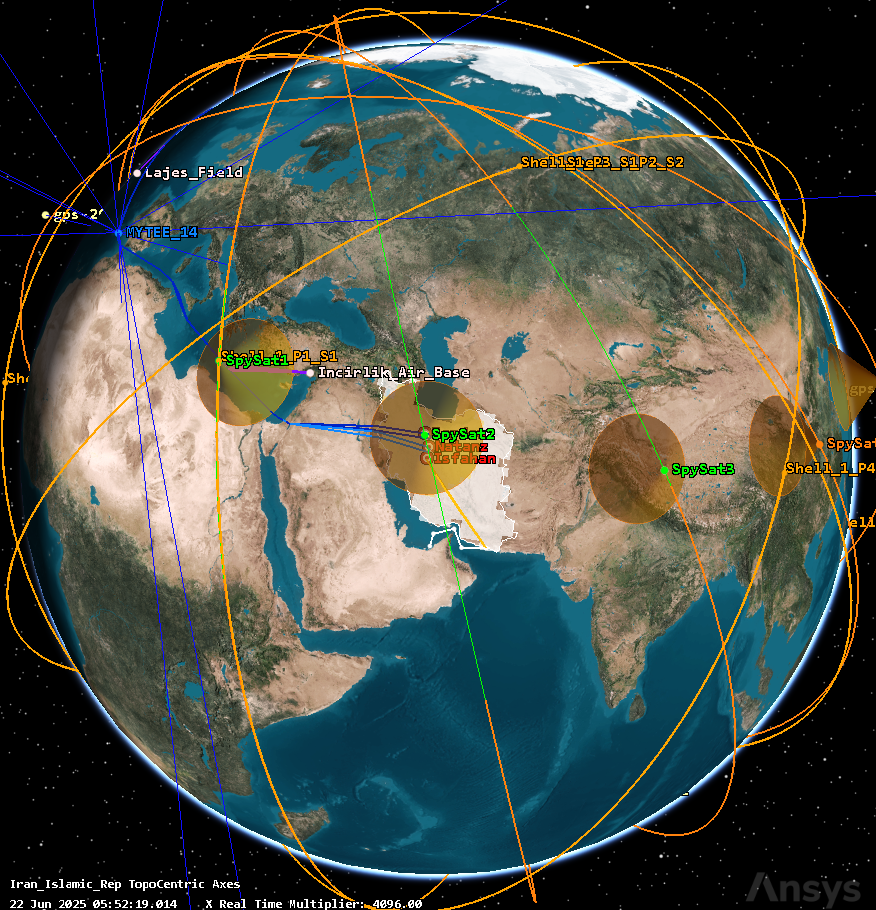
\includegraphics[width=\textwidth]{LaTeX/Figures/OpticalSpy3D.png}
        \caption{3D graphic window of optical spysat pass.}
        \label{fig:3d_spysat}
    \end{subfigure}
    
\end{figure}

\subsubsection{Infrared Satellites}

The infrared satellites were modelled using a \texttt{Walker constellation} in STK. We generated the satellite collection using 5 planes and 2 shells per plane emanating from a seed satellite at \SI{500}{\kilo\metre} altitude, for a total of 10 infrared satellites. This orbit is suitable because LEO allows for effective infrared imaging and quick data transmission, with low latency compared to higher orbits. Their inclinations were optimised for coverage over mid-latitudes, where the Iranian sites are located, ensuring efficient passes without wasting time over irrelevant areas. A Walker pattern distributes the satellites evenly, minimising gaps in monitoring. This is enabled by our careful choice of the separation parameter between adjacent orbits, which were fine-tuned to produce a ``cross" pattern over the nuclear facilities in Iran for each pair of in-plane satellites. Figure~\ref{fig:infrared_pass} shows an overhead pass of one of these satellites over the desired target region, illuminating the surface facility pixels of the target. The ``cross" pattern is clearly visible, and the second in-plane satellite (on the other branch of the cross) is due to pass shortly afterwards. 

\begin{figure}
    \centering
    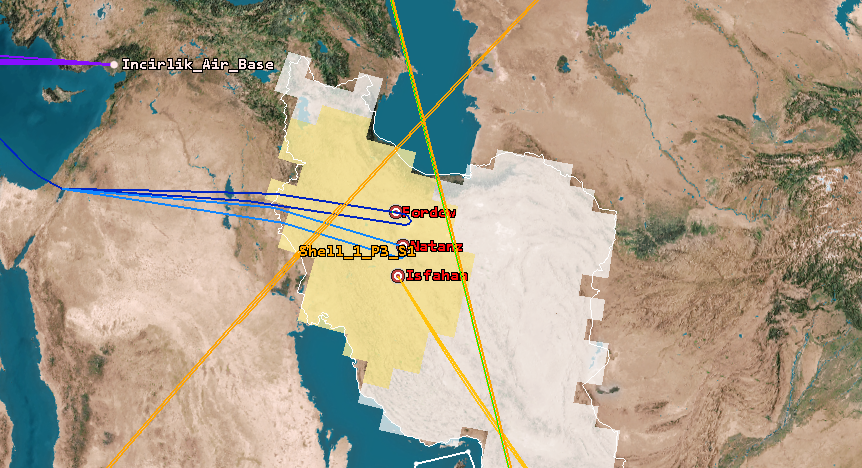
\includegraphics[width=\linewidth]{LaTeX/Figures/InfraredSatPAss.png}
    \caption{3D window of an overhead pass of the infrared HammerEye satellite.}
    \label{fig:infrared_pass}
\end{figure}

\subsubsection{Figure of Merit}

Finally, a \texttt{Figure of Merit} object was attached to the CoverageDefinition defined above. This figure of merit was used to compute the coverage results discussed in the following section. This figure of merit was computed over the period ranging from 22nd June 2025 at 04:30:00 UTC (corresponding to the first arrival of the optical imaging satellites overhead of the target facility), and spanned a 2-hour long period, ending on 22nd June 2025 at 06:30:00 UTC.

\subsection{Results}

\begin{figure}[h]
    \centering
    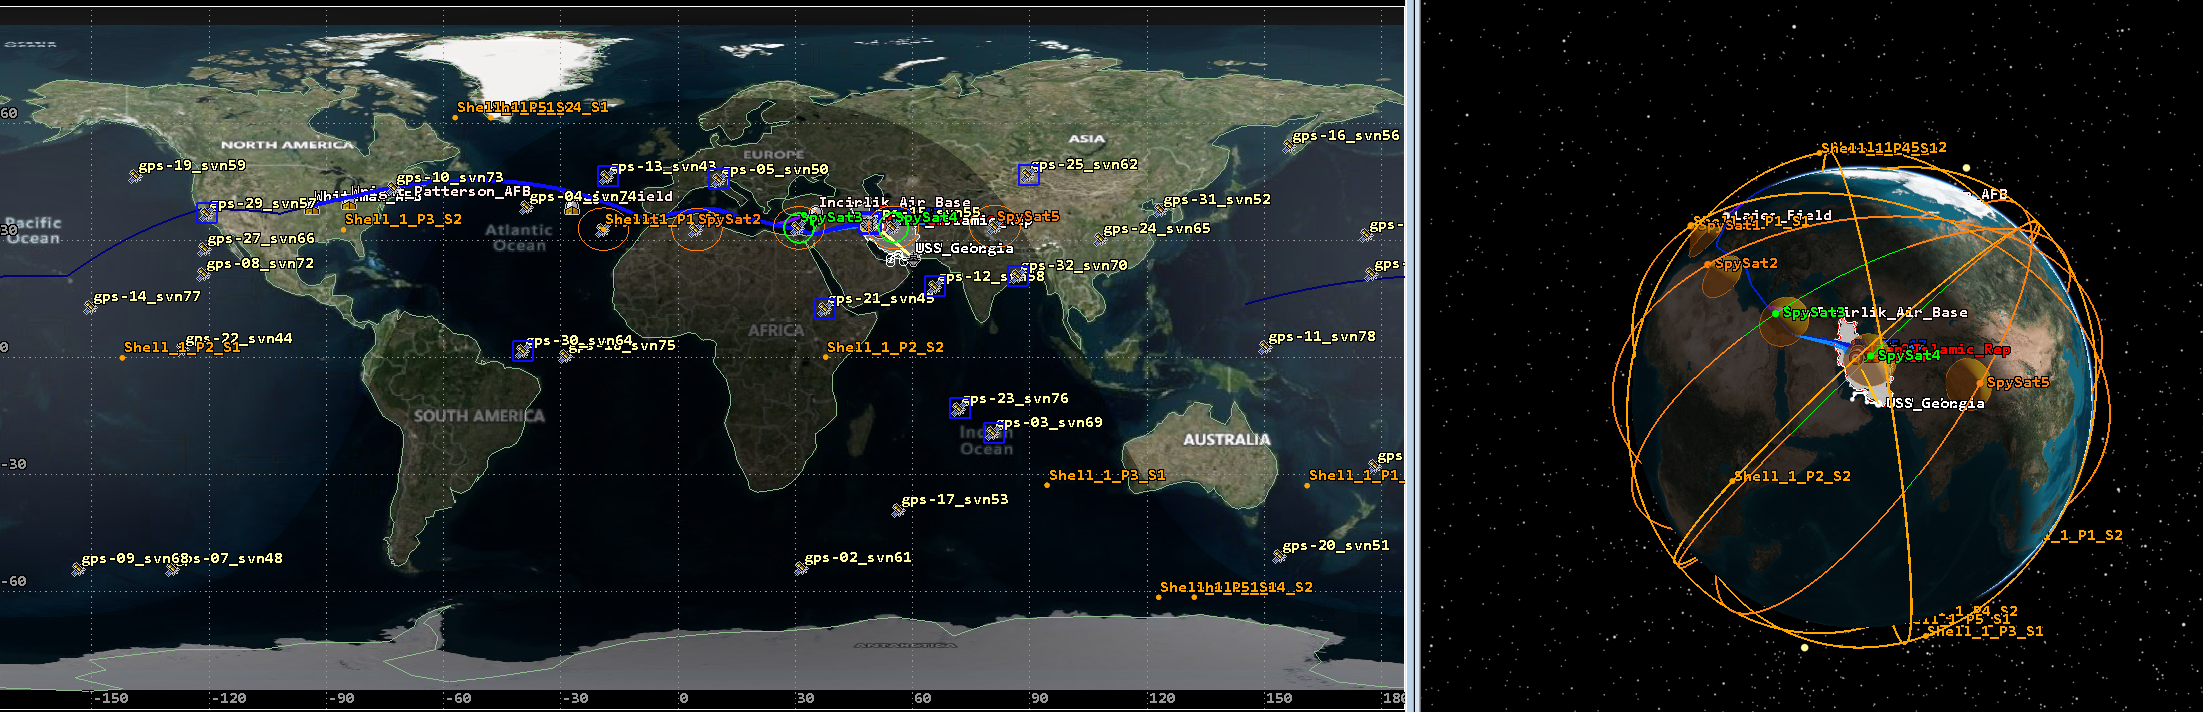
\includegraphics[width=\linewidth]{LaTeX/Figures/FinalResuult.png}
    \caption{Final state of the HammerEye constellation and the STK model. 2D window (left), 3D (right).}
    \label{fig:final_result}
\end{figure}

We provide both the 2D and the 3D view window of our finalised HammerEye satellite constellation (as well as the objects from the original OMH mission) in Figure~\ref{fig:final_result}.

Additionally, figure of merit plots for total access over the two hour window, plotted over Latitude and Longitude values, are displayed in Figure~\ref{fig:latitude} and Figure~\ref{fig:longitude}, respectively. These figures shows the requirement of achieving over 50 percent coverage is indeed achieved. The HammerEye espionage system design is a powerful extension to the original OMH, permitting the US military to monitor the state of critical assets in Iranian territory without risking any assets or ground troops. Our model shows that, even with a simple and inexpensive 15-satellite design, a satisfactory coverage rate can be achieved, providing both optical and infrared imagery and intelligence over the region. At the current state of modern warfare capabilities, there are no known weapons possessed by Iran which could threaten the operability and functioning of the HammerEye system, thereby ensuring a long-term solution for keeping the Iranian nuclear program in check, and strengthening the impact of OMH's strikes and overall mission.
\begin{figure}[h]
    \centering
    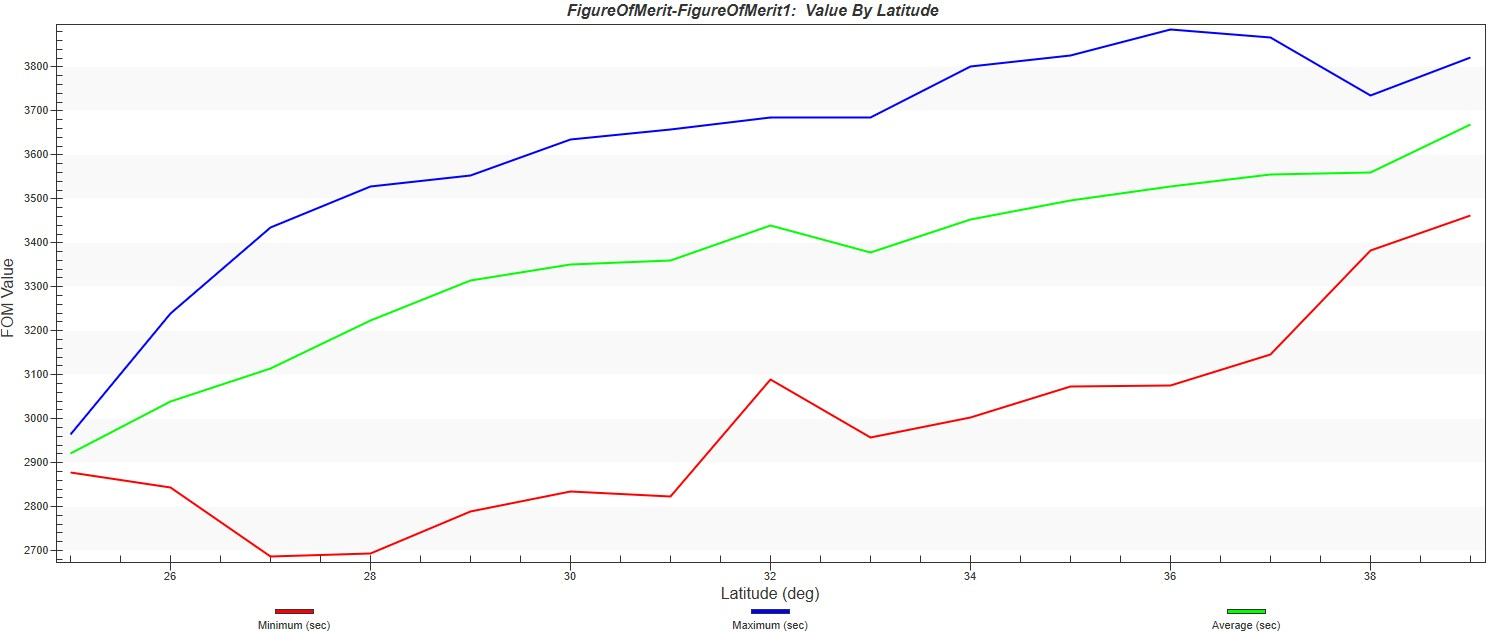
\includegraphics[width=\linewidth]{LaTeX/Figures/FigureOfMerit1_Value_By_Latitude.jpg}
    \caption{Values of the figure of merit over the CoverageDefinition on Iran varying by Latitude.}
    \label{fig:latitude}
\end{figure}

\begin{figure}[h]
    \centering
    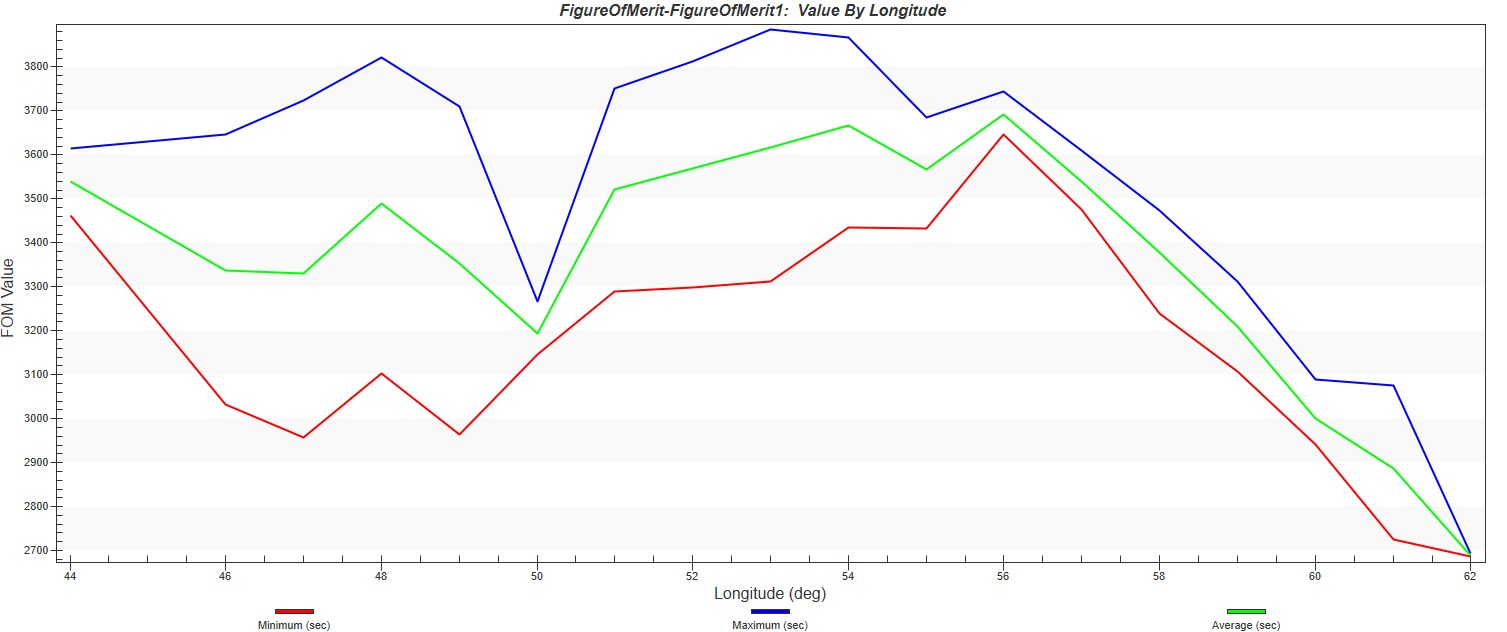
\includegraphics[width=\linewidth]{LaTeX/Figures/FigureOfMerit1_Value_By_Longitude.jpg}
    \caption{Values of the figure of merit over the CoverageDefinition on Iran varying by Longitude.}
    \label{fig:longitude}
\end{figure}



\subsection{Updated STK Model}

A link to the video of the updated STK simulation is provided on Canvas. The video shows the constellation in operation, with sensor footprints covering the sites and access links to the coverage definition lighting up the white squares orange. The video also confirms the constellation design satisfied the mission requirements as an extension of OMH.


\subsection{Discussion and Interpretation}
Compared to Part A, this extension shifts focus from immediate strikes to sustained space operations, requiring trade-offs such as balancing constellation size for better coverage against higher costs. The design worked well, with HPOP accurately modelling the orbits in the scenario window. In terms of realism, operational versions would need hardened electronics against radiation and coordination with allies for ground support. What changed most was the addition of sophisticated imaging and intelligence space assets, strenghtening the original implementation which only contained one LEO electro-optical satellite for imaging. Next steps might include integrating with existing networks, like the Space Development Agency's tracking layer, to enhance anti-jamming capabilities. Overall, this extension highlights space's role in multi-domain warfare, making the mission more robust.

\fi

\section{Conclusion} \label{sec:conclusion}
\ifpartB
\subsection{Original Mission}
\fi
This document presented a model of Operation Midnight Hammer in STK. Apart from classified or otherwise inaccessible information, to the best of the authors' knowledge, this model reproduced precisely the unfolding of the operation, following each critical mission phase with minute accuracy. The model highlighted several of the mission's tradeoffs: first, we noted that, although the US has capable supersonic aircraft, the mission was carried out by subsonic B-2 bombers to prioritise stealth over mission duration. The mission lasted 37 hours in total, which was demanding for the 14 pilots involved, but it also ensured that US forces maintained the element of surprise. Secondly, reliance on extensive aerial refuelling, which occurred six times with tankers from Wright-Patterson Air Force Base in Ohio, Lajes Field in the Azores, and Incirlik Air Base in Türkiye, introduced operational complexity and heightened the risk of detection. However, this approach enabled global reach without the need for forward basing, thereby mitigating geopolitical tensions. The project also highlighted the meticulous planning required to execute such a complex mission, and the central role that satellite intelligence plays in coordinating so many aircraft, ships, missiles and ground facilities. Coordinating aerial strikes with maritime missile launches over several thousand kilometres, with no direct line of sight due to Earth's curvature, is only possible with the aid of lightspeed satellite communications. These mission details often go unnoticed in press coverage of military operations, despite their fundamental role.

\ifpartB
\subsection{Extension}
Overall, this updated mission design draws from real space espionage US and NASA programs. It is highly likely, in fact, that a very similar constellation was actually deployed to analyse and spy on the Iranian nuclear programme after OMH. It goes without saying that access to any details on such a programme are not granted to the general public. Due to this, we note that our model is therefore only an approximation (although a faithful one). A total of 60 hours of work time were spent on modelling each of the aircraft, ships, satellites, constellations, collections, missiles, facilities, targets, coverages, and sensor objects. In fact, the project involved 11 out of the 14 principal STK objects, demanding a broad training on several Ansys tutorials, and enabling the in-depth exploration of the software's capabilities. 
\fi
Throughout this project, I developed a profound appreciation for the coordination and operational capabilities of the US Air Force, and a deep understanding of how these missions are facilitated through the use of satellites. As an enthusiast on military operations and assets---especially those of the united states---I have never been exposed to the level of intricacy required in planning a mission as complicated as OMH. Even just by simulating the mission in STK, without any stakes or human lives on the line, turned out to be an incredibly stimulating challenge in careful planning and meticulous mission timing.
\ifpartB
Furthermore, the extension involving the HammerEye constellation, which solidified the mission's main objective by providing extensive coverage and intelligence over the struck nuclear sites, enriched my respect for planning out the deployment of satellite constellations and pushed me to explore an even broader range of STK tools and objects. I have really enjoyed working on this project, and personally (as an Oxford student on my first semester at Princeton) this project has represented the most stimulating and compelling assignment in my undergraduate career.
\fi

\clearpage
\printbibliography


\end{document}
